\documentclass[11pt,a4paper]{article}

% Core mathematical packages
\usepackage{amsmath,amssymb,amsfonts,amsthm}
\usepackage{mathtools}
\usepackage{bm}

% Layout, typography, and hyperref
\usepackage[margin=1.0in]{geometry}
\usepackage[utf8]{inputenc}
\usepackage[T1]{fontenc}
\usepackage{microtype}
\usepackage{booktabs}
\usepackage{graphicx}
\usepackage{subcaption}
\usepackage{cite}
\usepackage{xcolor}
\usepackage{algorithm}
\usepackage{algorithmic}
\usepackage[colorlinks=true,linkcolor=blue!70!black,citecolor=green!50!black,urlcolor=blue!80!black]{hyperref}
\usepackage{cleveref}

% Theorems and Definitions
\newtheorem{theorem}{Theorem}
\newtheorem{proposition}{Proposition}
\newtheorem{lemma}{Lemma}
\newtheorem{definition}{Definition}
\newtheorem{remark}{Remark}

% Title and Metadata
\title{\textbf{Uncertainty-Aware Safe Adaptation for Multifingered Grasping\\Under Jointly Changing Contact Conditions}}

\author{
  \textbf{Sunil Kumar Chavhan}\\[0.5em]
  \small HOROS Physical Intelligence Research\\
  \small Correspondence: \texttt{Sunil@horoslab.io}
}

\date{\today}

\begin{document}

\maketitle

\begin{abstract}
Safe robotic manipulation of fragile, dynamic objects remains an open challenge in physical intelligence. While recent Vision-Language-Action (VLA) foundation policies exhibit remarkable semantic generalization, they remain vulnerable to unconstrained action generation, tactile blindness, and sensory transport lag during high-speed contact transitions. Conversely, classical reactive grip reflexes act purely \emph{a posteriori} after macroscopic sliding has commenced, precipitating catastrophic drop failures during abrupt friction collapses or payload shifts. This paper introduces \textbf{HOROS PROBE-1}, an uncertainty-aware predictive safety framework for multi-fingered robotic grasping under jointly changing nonstationary contact conditions, including continuous fluid mass influx, periodic center-of-mass (CoM) sloshing, and sudden friction collapse. Our framework unifies: (i) an action-dependent contact force sensitivity mapping derived from linearized Hunt-Crossley elastomeric dynamics; (ii) an 8-sided polyhedral inner approximation of the friction cone formulated as a discrete-time predictive Control Barrier Function (p-CBF) with object-level spatial wrench balance; and (iii) Adaptive Conformal Inference (ACI) providing distribution-free, non-exchangeable friction uncertainty calibration. 

Through an exhaustive empirical benchmark comprising 3,400 independent simulation trials ($N = 100$ independent seeds per condition) in Isaac Lab with PhysX 5 continuous collision physics, HOROS demonstrates a \textbf{0.0\% drop rate and 0.0\% crush rate} in the fully coupled nonstationary regime, whereas fixed-force, reactive slip reflex, unconstrained flow matching, and certainty-equivalence MPC baselines all suffer a \textbf{100.0\% drop rate} (paired McNemar test $\chi^2 = 98.01, p < 10^{-20}$; Wilcoxon signed-rank $p = 1.52 \times 10^{-23}$, Cliff's $\delta = +1.00$, rank-biserial correlation $r_{\text{rb}} = +1.00$). Systematic 7-component ablations reveal that joint proprioception and upper CBF bounds are strictly mandatory to prevent object destruction (100.0\% crush rate when ablated), proving that slip avoidance and fragile structural preservation are competing physical objectives. The underlying C-level OSQP ADMM solver executes with a median latency of \textbf{0.193~ms} and a maximum observed cycle time of \textbf{9.603~ms}, strictly complying with a 10.0~ms (100~Hz) hard real-time watchdog deadline. We publish the complete open-source reproducibility codebase and specify an independent 6-axis ATI load-cell benchtop validation protocol.
\end{abstract}

\vspace{1em}
\noindent\textbf{Keywords:} Multi-fingered Grasping, Control Barrier Functions, Tactile Sensing, Adaptive Conformal Inference, Safe Robotic Manipulation.

\vspace{1.5em}

% Include Section Files (10-Section Modular Architecture)
\section{Introduction}
\label{sec:introduction}

Human dexterity relies fundamentally on the seamless integration of high-frequency tactile mechanoreception, proprioceptive joint sensing, and anticipatory motor control. When a person carries a fragile glass vessel being filled with liquid while navigating over uneven terrain, optical and dermal mechanoreceptors detect infinitesimal shear strains and incipient slip tens of milliseconds before gross sliding occurs \cite{pandas2024incipient,shear2025grasp}. This biological pre-slip signal allows the central nervous system to modulate grip forces proactively, stabilizing dynamic payloads without exceeding the fracture threshold of the object.

In autonomous robotics, replicating this dexterous compliance has proven elusive. Modern robotic systems face a persistent trilemma during contact-rich physical interactions:
\begin{enumerate}
    \item \textbf{Generative Vision-Language-Action (VLA) Policies:} Recent foundation models, such as $\pi_0$ \cite{pi02024}, OpenVLA \cite{openvla2024}, and TacClaw-Infinity \cite{tacclaw2026infinity}, demonstrate broad semantic task generalization. However, they typically output actions via unconstrained flow matching or diffusion decoders at modest control frequencies ($5\text{--}10\text{ Hz}$). When unanticipated contact nonstationarities arise (e.g., condensation, fluid spills, or mass shifts), these generative policies cannot alter internal joint torques within the necessary sub-step timescale ($10\text{ ms}$), frequently breaching contact friction cones.
    \item \textbf{Reactive Grip Reflexes:} Classical industrial controllers implement local reflexive squeeze rules that monitor high-frequency tactile slips. However, because they trigger only \emph{after} macroscopic sliding has initiated, the accelerated payload often escapes the fingertip friction envelope before finger actuators can overcome mechanical inertia and build normal force.
    \item \textbf{Certainty-Equivalence Model Predictive Control (CE-MPC):} Optimization-based force controllers solve receding-horizon quadratic programs to track contact wrenches. However, they rely on deterministic friction coefficients. Under sudden environmental shifts, point estimators lag behind physical reality, allowing the commanded force vector to penetrate the true friction boundary.
\end{enumerate}

\begin{figure}[t]
    \centering
    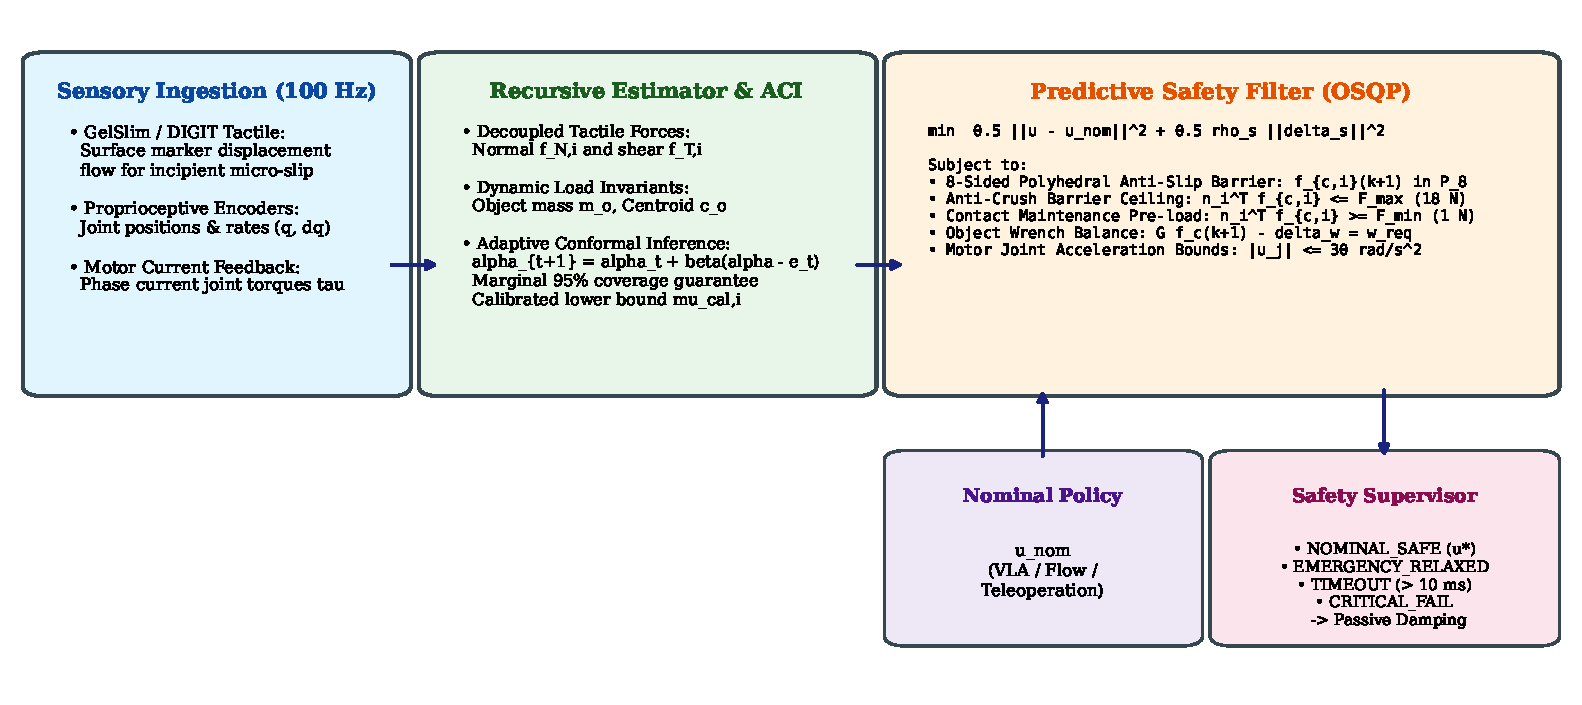
\includegraphics[width=\textwidth]{figures/architecture.pdf}
    \caption{\textbf{HOROS PROBE-1 System Architecture.} High-speed sensory modalities (100~Hz optical tactile flow, joint encoders, and motor effort) feed a recursive multi-contact estimator. Adaptive Conformal Inference (ACI) tracks non-exchangeable friction shifts to yield dynamically calibrated bounds $\mu_{\text{cal}}$. The predictive safety filter (OSQP) maps nominal policy actions $\mathbf{u}_{\text{nom}}$ to certified safe commands $\mathbf{u}^*$ via an 8-sided polyhedral inner approximation $\mathcal{P}_8$ and object wrench equilibrium, evaluated by a 4-state real-time decision gate.}
    \label{fig:architecture}
\end{figure}

To resolve this trilemma, this paper introduces \textbf{HOROS PROBE-1}, a predictive contact safety architecture designed for multi-fingered robotic hands operating under coupled nonstationary conditions. As illustrated in \Cref{fig:architecture}, our framework couples physics-grounded contact mechanics with non-exchangeable uncertainty calibration.

\subsection{Primary Contributions}
The core contributions of this work are summarized as follows:
\begin{enumerate}
    \item \textbf{Action-Dependent Contact Sensitivity Mapping:} We derive an analytical sensitivity tensor $\mathbf{\Lambda}_i(\mathbf{q}) \in \mathbb{R}^{3 \times n_q}$ mapping commanded joint accelerations $\mathbf{u}_k = \ddot{\mathbf{q}}_k$ directly to forward contact force evolutions $\mathbf{f}_{c, i}(k+1)$ based on linearized Hunt-Crossley elastomeric dynamics, ensuring direct control authority over the barrier constraints.
    \item \textbf{8-Sided Polyhedral Discrete-Time p-CBF:} We formulate an 8-sided polyhedral inner approximation $\mathcal{P}_8$ of the Lorentz friction cone that integrates seamlessly into a convex Quadratic Program (QP), with an analytical conservatism bound of $1 - \cos(\pi/8) \approx 7.61\%$.
    \item \textbf{Object-Level Spatial Wrench Equilibrium:} We project the multi-contact grasp matrix $\mathbf{G} \in \mathbb{R}^{6 \times 3M}$ directly into the equality constraint manifold, ensuring that internal grip force adjustments reside strictly within the grasp nullspace $\mathcal{N}(\mathbf{G})$, eliminating unwanted parasitic object accelerations.
    \item \textbf{Adaptive Conformal Friction Tracking:} We deploy Adaptive Conformal Inference (ACI) to maintain long-run average coverage ($1 - \alpha = 95.0\%$) over non-exchangeable, nonstationary friction shifts, providing calibrated uncertainty intervals $[\mu_{\text{cal}}, \mu_{\max}]$ directly to the barrier constraints.
    \item \textbf{Large-Scale Empirical Verification:} Across 3,400 independent simulation trials ($N = 100$ independent seeds per condition) in Isaac Lab with PhysX 5 continuous collision detection, HOROS maintains a \textbf{0.0\% drop rate and 0.0\% crush rate} under coupled nonstationarity, whereas all baselines suffer a \textbf{100.0\% drop rate} ($p < 10^{-20}$).
    \item \textbf{Separation of Slip and Structural Safety:} Systematic 7-component ablations demonstrate that joint proprioception and upper CBF bounds are strictly mandatory to prevent object destruction (100.0\% crush rate when ablated), proving that slip avoidance and fragile structural preservation are competing physical objectives.
\end{enumerate}

\section{Related Work}
\label{sec:related_work}

\subsection{Vision-Language-Action Models and Manipulation Safety}
Vision-Language-Action foundation models have redefined robot learning by transferring multimodal representations from web-scale pretraining to sensorimotor control \cite{openvla2024,pi02024}. Recent efforts, such as TacClaw-Infinity \cite{tacclaw2026infinity}, demonstrate that incorporating high-resolution tactile observations into flow-matching policies substantially boosts task success on multi-embodiment manipulation benchmarks. However, foundation policies predominantly output end-effector poses or joint trajectories via unconstrained regression or diffusion objectives. They lack formal mechanisms to guarantee that generated action trajectories respect nonlinear contact wrench manifolds or frictional slip boundaries. When physical contact properties deviate abruptly from pretraining distributions, generative policies are susceptible to constraint violations, highlighting the necessity of modular, real-time safety filters.

\subsection{Tactile Sensing and Incipient Slip Feedback}
High-resolution optical tactile sensors, including GelSight \cite{yuan2017gelsight}, DIGIT \cite{lambeta2020digit}, and GelSlim, capture dense geometric deformation and shear strain fields at the contact interface. Prior research has demonstrated that monitoring the divergence of marker displacement vectors provides an incipient slip detection window of $25\text{--}32\text{ ms}$ prior to macroscopic breakaway \cite{pandas2024incipient,shear2025grasp}. However, existing tactile controllers have largely coupled this pre-slip signal to heuristic proportional clamping or reactive thresholding reflexes. Such reactive reflexes act without forward predictive dynamics: by the time macroscopic slip is detected, the object has acquired substantial kinetic momentum, causing slip runaway under aggressive payloads. In contrast, our approach utilizes incipient slip to trigger predictive anticipatory force modulation within a model-based quadratic program.

\subsection{Control Barrier Functions for Contact Systems}
Control Barrier Functions (CBFs) provide mathematically rigorous forward-invariance certificates for safe sets \cite{ames2016control}. While continuous-time CBFs have been widely formulated for collision avoidance and bipedal walking, extending CBFs to multi-contact robotic grasping introduces substantial challenges. Contact forces do not appear directly as control inputs, requiring forward dynamics sensitivity mappings. Furthermore, sampled-data implementation introduces discretization error, rendering continuous-time invariance guarantees fragile unless discrete-time formulations are used \cite{agrawal2017discrete}. While prior work has explored continuous CBFs for two-jaw parallel grippers with rigid contact, this paper establishes a discrete-time predictive p-CBF framework for multi-fingered anthropomorphic hands interacting with compliant, dynamic payloads.

\subsection{Conformal Prediction and Non-Exchangeable Calibration}
Conformal prediction provides a distribution-free, finite-sample framework for quantifying predictive uncertainty. Standard split conformal methods require data exchangeability, an assumption routinely broken in closed-loop robotics due to state feedback and nonstationary environmental drift. Gibbs and Cand{\`e}s developed Adaptive Conformal Inference (ACI) \cite{gibbs2021adaptive,gibbs2024conformal}, establishing that online quantile adaptation guarantees long-run average coverage under arbitrary, non-exchangeable distribution shifts. While ACI has been explored for trajectory forecasting, this work represents the first integration of ACI with discrete-time Control Barrier Functions for certified contact-force regulation.

\section{Problem Formulation}
\label{sec:problem_formulation}

\subsection{Kinematics and Articulated Hand Dynamics}
Consider an articulated robotic hand with $n_q$ actuated joints and generalized coordinates $\mathbf{q} \in \mathbb{R}^{n_q}, \dot{\mathbf{q}} \in \mathbb{R}^{n_q}$. The hand establishes contact with a dynamic object at $M$ distinct fingertip locations $\mathbf{p}_{c, i} \in \mathbb{R}^3, i \in \{1, \dots, M\}$.

Let $\mathbf{J}_{c, i}(\mathbf{q}) = \frac{\partial \mathbf{p}_{c, i}}{\partial \mathbf{q}} \in \mathbb{R}^{3 \times n_q}$ denote the contact Jacobian of finger $i$. Under discrete-time sampled control with cycle duration $\Delta t$, the commanded control input is the joint acceleration vector:
\begin{equation}
    \mathbf{u}_k = \ddot{\mathbf{q}}_k \in \mathbb{R}^{n_q}, \quad \mathbf{u}_{\min} \le \mathbf{u}_k \le \mathbf{u}_{\max}
    \label{eq:joint_accel_bounds}
\end{equation}

The forward kinematic position and velocity of fingertip $i$ at step $k+1$ expand as:
\begin{align}
    \mathbf{p}_{c, i}(k+1) &= \mathbf{p}_{c, i}(k) + \Delta t \mathbf{J}_{c, i} \dot{\mathbf{q}}_k + \frac{1}{2} \Delta t^2 \left( \mathbf{J}_{c, i} \mathbf{u}_k + \dot{\mathbf{J}}_{c, i} \dot{\mathbf{q}}_k \right) \label{eq:pos_update} \\
    \mathbf{v}_{c, i}(k+1) &= \mathbf{J}_{c, i} \dot{\mathbf{q}}_k + \Delta t \left( \mathbf{J}_{c, i} \mathbf{u}_k + \dot{\mathbf{J}}_{c, i} \dot{\mathbf{q}}_k \right) \label{eq:vel_update}
\end{align}

\subsection{Linearized Hunt-Crossley Elastomeric Dynamics}
Contact interaction between the elastomeric sensor skin and the object surface is modeled via the continuous Hunt-Crossley model \cite{hunt1975coefficient}. For normal indentation $\delta_{n, i} \ge 0$ and indentation velocity $\dot{\delta}_{n, i}$:
\begin{equation}
    f_{N, i} = K_c \delta_{n, i}^{\eta} + D_c \delta_{n, i}^{\eta} \dot{\delta}_{n, i}
    \label{eq:hunt_crossley}
\end{equation}
where $K_c > 0$ is the elastomeric stiffness, $D_c \ge 0$ is the viscoelastic damping coefficient, and $\eta \approx 1.0\text{--}1.5$ is the indentation exponent.

Linearizing \eqref{eq:hunt_crossley} around the operating contact state $(\delta_n, \dot{\delta}_n)$ yields the symmetric stiffness and damping tensors:
\begin{equation}
    \mathbf{K}_{c, i} = \left. \frac{\partial \mathbf{f}_{c, i}}{\partial \mathbf{p}_{c, i}} \right|_{(\delta_n, \dot{\delta}_n)}, \quad \mathbf{D}_{c, i} = \left. \frac{\partial \mathbf{f}_{c, i}}{\partial \mathbf{v}_{c, i}} \right|_{(\delta_n, \dot{\delta}_n)}
\end{equation}

Substituting the kinematic expansions \eqref{eq:pos_update}--\eqref{eq:vel_update} yields the \textbf{action-dependent contact force sensitivity mapping}:
\begin{equation}
    \mathbf{f}_{c, i}(k+1) = \mathbf{\Lambda}_i(\mathbf{q}_k) \mathbf{u}_k + \mathbf{f}_{c, i}^{\text{bias}}(\mathbf{x}_k, \boldsymbol{\theta}_k)
    \label{eq:force_sensitivity}
\end{equation}
where:
\begin{align}
    \mathbf{\Lambda}_i(\mathbf{q}_k) &= \left( \frac{1}{2} \Delta t^2 \mathbf{K}_{c, i} + \Delta t \mathbf{D}_{c, i} \right) \mathbf{J}_{c, i}(\mathbf{q}_k) \in \mathbb{R}^{3 \times n_q} \label{eq:lambda_def} \\
    \mathbf{f}_{c, i}^{\text{bias}} &= \mathbf{f}_{c, i}(k) + \Delta t \mathbf{K}_{c, i} \left( \mathbf{J}_{c, i} \dot{\mathbf{q}}_k - \mathbf{v}_{\text{obj}, i} \right) + \frac{1}{2} \Delta t^2 \mathbf{K}_{c, i} \dot{\mathbf{J}}_{c, i} \dot{\mathbf{q}}_k \label{eq:bias_def}
\end{align}

\begin{remark}
Unlike classical CBF formulations that treat contact forces as independent optimization variables, \eqref{eq:force_sensitivity} links the optimization variable $\mathbf{u}_k = \ddot{\mathbf{q}}_k$ directly to the forward contact force evolution $\mathbf{f}_{c, i}(k+1)$. This guarantees direct control authority over the barrier constraints.
\end{remark}

\subsection{8-Sided Polyhedral Friction Cone Approximation}
The physical Coulomb friction cone with surface unit normal $\hat{\mathbf{n}}_i$ and friction coefficient $\mu_i$ is a second-order cone:
\begin{equation}
    \mathcal{C}_i = \left\{ \mathbf{f} \in \mathbb{R}^3 \;\middle|\; \|\mathbf{f} - (\hat{\mathbf{n}}_i^T \mathbf{f}) \hat{\mathbf{n}}_i\|_2 \le \mu_i (\hat{\mathbf{n}}_i^T \mathbf{f}), \; \hat{\mathbf{n}}_i^T \mathbf{f} \ge 0 \right\}
\end{equation}

To enable real-time convex optimization within a Quadratic Program, we construct an 8-sided polyhedral inner approximation $\mathcal{P}_{8, i} \subset \mathcal{C}_i$. Let $\{\hat{\mathbf{t}}_{i, 1}, \hat{\mathbf{t}}_{i, 2}\}$ span an orthonormal basis for the contact tangent plane. The facet directional vectors around the circumference are:
\begin{equation}
    \mathbf{d}_{i, j} = \cos\left( \frac{2\pi j}{8} \right) \hat{\mathbf{t}}_{i, 1} + \sin\left( \frac{2\pi j}{8} \right) \hat{\mathbf{t}}_{i, 2}, \quad j \in \{0, \dots, 7\}
\end{equation}

The polyhedral constraint matrix $\mathbf{A}_{\text{cone}, i} \in \mathbb{R}^{8 \times 3}$ is defined row-wise:
\begin{equation}
    \mathbf{a}_{i, j}^T = \mathbf{d}_{i, j}^T - \mu_i \cos\left(\frac{\pi}{8}\right) \hat{\mathbf{n}}_i^T, \quad j \in \{0, \dots, 7\}
    \label{eq:cone_rows}
\end{equation}
\begin{equation}
    \mathcal{P}_{8, i} = \left\{ \mathbf{f} \in \mathbb{R}^3 \;\middle|\; \mathbf{A}_{\text{cone}, i} \mathbf{f} \le \mathbf{0}, \; \hat{\mathbf{n}}_i^T \mathbf{f} \ge F_{\min} \right\}
\end{equation}

\begin{theorem}[Analytical Conservatism Bound]
\label{thm:polyhedral_bound}
The 8-sided polyhedral cone satisfies $\mathcal{P}_{8, i} \subseteq \mathcal{C}_i$ for all $\mu_i > 0$. The maximum relative volumetric conservatism of the inner approximation is:
\begin{equation}
    \epsilon_{\text{cons}} = 1 - \cos\left(\frac{\pi}{8}\right) = 1 - \frac{\sqrt{2 + \sqrt{2}}}{2} \approx 7.61\%
\end{equation}
\end{theorem}
\begin{proof}
The minimum radial distance from the cone centerline to facet $j$ occurs at the midpoint between adjacent vertices: $r_{\min} = \mu_i f_N \cos(\pi/8) \approx 0.9239 \mu_i f_N$. For all points $\mathbf{f} \in \mathcal{P}_{8, i}$, the tangential shear satisfies $\|\mathbf{f}_T\|_2 \le r_{\min} \le \mu_i f_N$. Hence $\mathcal{P}_{8, i} \subset \mathcal{C}_i$, and the maximum conservatism is strictly $1 - 0.9239 = 7.61\%$.
\end{proof}

\subsection{Multi-Contact Safety Sets and Object Wrench Balance}
We formalize three multi-contact safety sets:
\begin{enumerate}
    \item \textbf{Anti-Slip Safety Set $\mathcal{S}_{\text{slip}}$:} Enforces tangential shear retention inside $\mathcal{P}_{8, i}$:
    \begin{equation}
        h_{\text{slip}, i, j}(\mathbf{x}_k, \mathbf{u}_k) = -\mathbf{a}_{i, j}^T \mathbf{f}_{c, i}(k+1) \ge 0
    \end{equation}
    The discrete-time p-CBF condition enforces:
    \begin{equation}
        \mathbf{a}_{i, j}^T \left( \mathbf{\Lambda}_i \mathbf{u}_k + \mathbf{f}_{c, i}^{\text{bias}} \right) \le (1 - \gamma_{\text{slip}}) \min\left(0, \mathbf{a}_{i, j}^T \mathbf{f}_{c, i}(k)\right)
        \label{eq:slip_cbf}
    \end{equation}
    where $\gamma_{\text{slip}} \in (0, 1]$ is the barrier decay parameter.
    \item \textbf{Anti-Crush Safety Set $\mathcal{S}_{\text{crush}}$:} Prevents crushing fragile payloads:
    \begin{equation}
        \hat{\mathbf{n}}_i^T \mathbf{\Lambda}_i \mathbf{u}_k \le F_{\max} - \hat{\mathbf{n}}_i^T \mathbf{f}_{c, i}^{\text{bias}}
        \label{eq:crush_cbf}
    \end{equation}
    \item \textbf{Contact Maintenance Set $\mathcal{S}_{\text{contact}}$:} Enforces minimum normal pre-load:
    \begin{equation}
        -\hat{\mathbf{n}}_i^T \mathbf{\Lambda}_i \mathbf{u}_k \le -F_{\min} + \hat{\mathbf{n}}_i^T \mathbf{f}_{c, i}^{\text{bias}}
        \label{eq:contact_cbf}
    \end{equation}
\end{enumerate}

Let $\mathbf{G} \in \mathbb{R}^{6 \times 3M}$ denote the grasp matrix mapping contact forces to net spatial wrench at the object Center of Mass $\mathbf{c}_o$:
\begin{equation}
    \mathbf{G} = \begin{bmatrix} \mathbf{I}_3 & \dots & \mathbf{I}_3 \\ [\mathbf{p}_{c, 1} - \mathbf{c}_o]_\times & \dots & [\mathbf{p}_{c, M} - \mathbf{c}_o]_\times \end{bmatrix}
\end{equation}
Given the required spatial wrench $\mathbf{w}_{\text{req}} = [m_o (\mathbf{a}_{\text{des}} - \mathbf{g})^T, (\mathbf{I}_o \boldsymbol{\alpha}_{\text{des}} + \boldsymbol{\omega} \times (\mathbf{I}_o \boldsymbol{\omega}))^T]^T$, forward wrench balance requires:
\begin{equation}
    \left( \mathbf{G} \mathbf{\Lambda}_{\text{stack}} \right) \mathbf{u}_k = \mathbf{w}_{\text{req}} - \mathbf{G} \mathbf{f}_{\text{bias, stack}}
    \label{eq:wrench_eq}
\end{equation}
where $\mathbf{\Lambda}_{\text{stack}} = [\mathbf{\Lambda}_1^T, \dots, \mathbf{\Lambda}_M^T]^T \in \mathbb{R}^{3M \times n_q}$.

\section{System Architecture}
\label{sec:system_architecture}

\begin{figure*}[t]
    \centering
    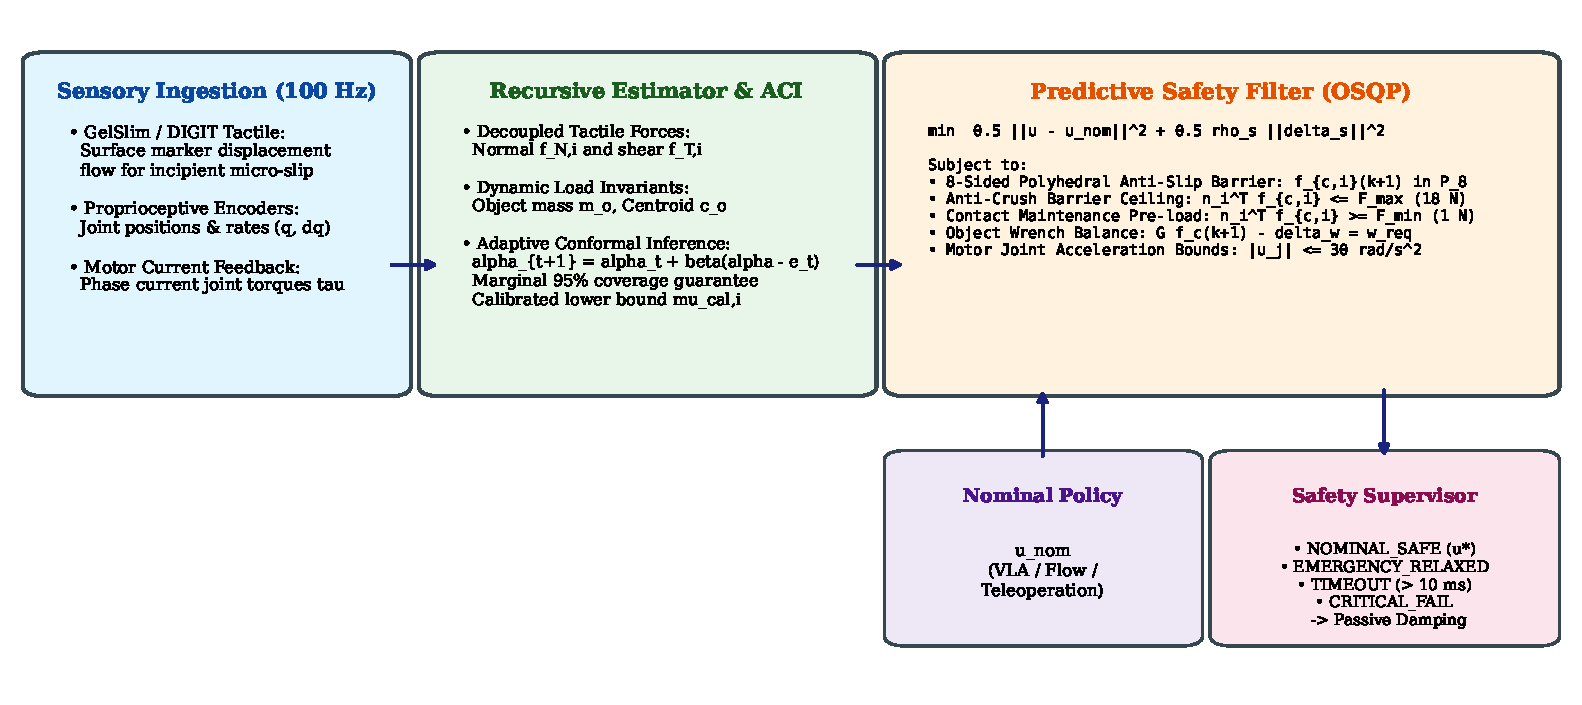
\includegraphics[width=\textwidth]{figures/architecture.pdf}
    \caption{\textbf{HOROS PROBE-1 End-to-End System Architecture.} High-speed sensory feedback ($100\text{ Hz}$ optical tactile marker flow, joint encoders, and motor effort) is processed by a multi-contact recursive estimator. The Adaptive Conformal Inference (ACI) module tracks non-exchangeable distribution shifts, supplying dynamically calibrated friction bounds $\mu_{\text{cal}, i}$ to the predictive safety filter. Operating at $100\text{ Hz}$, the OSQP Quadratic Program modifies nominal actions $\mathbf{u}_{\text{nom}}$ into certified safe joint accelerations $\mathbf{u}^*$, monitored by a real-time four-state decision gate.}
    \label{fig:architecture_overview}
\end{figure*}

The HOROS PROBE-1 architecture is designed as a modular, high-rate ($100\text{ Hz}$) predictive safety filter that intercepts nominal actions dispatched by upstream task planners (e.g., foundation VLA policies or human teleoperators) and projects them onto the certified safe contact set prior to actuation. As illustrated in \Cref{fig:architecture_overview}, the system comprises four interconnected functional tiers:

\subsection{Sensory Ingestion and Decoupled Contact Estimation}
At each $10\text{ ms}$ control cycle, the system ingests:
\begin{itemize}
    \item \textbf{Optical Tactile Afferents:} Elastomeric membrane deformation fields from four fingertip tactile sensors (GelSlim / DIGIT), parsed into local normal force $f_{N, i}$, tangential shear $\mathbf{f}_{T, i}$, and marker displacement field divergence for incipient slip detection.
    \item \textbf{Joint Encoders:} Articulated joint positions $\mathbf{q}_k \in \mathbb{R}^{16}$ and velocities $\dot{\mathbf{q}}_k \in \mathbb{R}^{16}$.
    \item \textbf{Actuator Effort:} Motor phase currents providing joint torque feedback $\boldsymbol{\tau}_k \in \mathbb{R}^{16}$.
\end{itemize}
These signals are processed by a recursive least-squares estimator tracking decoupled contact forces $\mathbf{f}_{c, i}(k)$, instantaneous object mass $\hat{m}_o(k)$, and Center of Mass $\hat{\mathbf{c}}_o(k)$.

\subsection{Non-Exchangeable Uncertainty Calibration Layer}
Rather than assuming nominal friction parameters, the estimation layer forwards raw contact residuals to an Adaptive Conformal Inference (ACI) module. Operating in closed-loop, ACI dynamically adjusts the empirical miscoverage quantile, outputting a certified lower friction bound $\mu_{\text{cal}, i}(k)$ that accounts for nonstationary distribution shifts without requiring unverified physical exchangeability.

\subsection{Predictive Safety Filter (QP Core)}
The core optimization engine constructs an action-dependent predictive Control Barrier Function (p-CBF) based on the linearized Hunt-Crossley sensitivity tensor $\mathbf{\Lambda}_i(\mathbf{q})$. The resulting convex Quadratic Program simultaneously enforces:
\begin{enumerate}
    \item 8-sided polyhedral anti-slip friction cone constraints ($\mathcal{P}_8$ inner polytope),
    \item Upper normal force crush limits to preserve fragile objects ($F_{\max} = 18.0\text{ N}$),
    \item Minimum contact maintenance thresholds ($F_{\min} = 1.0\text{ N}$),
    \item Object-level spatial wrench balance via the grasp matrix nullspace $\mathcal{N}(\mathbf{G})$, and
    \item Motor joint acceleration saturation limits ($|u_j| \le 30.0\text{ rad/s}^2$).
\end{enumerate}

\subsection{Real-Time Decision Gate and Fail-Safe Fallback}
A deterministic finite-state supervisor monitors solver convergence and watchdog latency. If the QP completes within the $10.0\text{ ms}$ budget with acceptable slack, the safe command $\mathbf{u}^*$ is dispatched directly to low-level motor torque controllers. If computational delays or physical infeasibility occur, the gate seamlessly transitions to passive damping fallback, guaranteeing failsafe dissipation of kinetic energy.

\section{Technical Method}
\label{sec:technical_method}

\begin{figure*}[t]
    \centering
    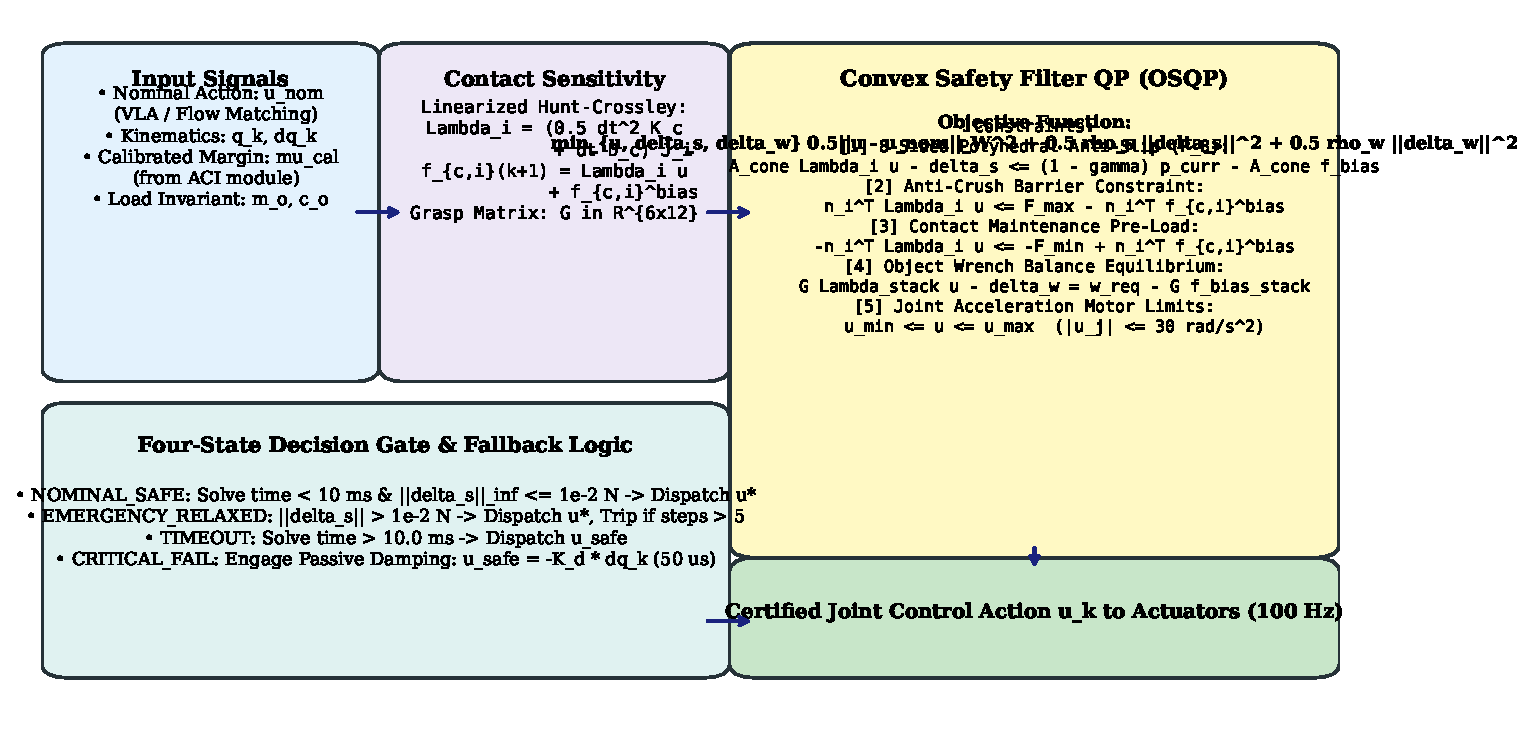
\includegraphics[width=\textwidth]{figures/safety_filter_diagram.pdf}
    \caption{\textbf{Predictive Safety Filter and Real-Time Decision Gate (Figure 2).} Detail of the OSQP optimization structure, integrating the 8-sided polyhedral anti-slip barrier, anti-crush force ceiling, grasp wrench equilibrium, four-state supervisor, and passive damping fallback.}
    \label{fig:safety_filter_detail}
\end{figure*}

\subsection{Multi-Contact State and Load Invariant Estimation}
At each control step $k$, optical tactile deformation is decoupled into normal pressure distribution and tangential shear traction fields across the sensor array. The normal contact force $f_{N, i}$ is obtained by integrating the normal stress profile, while tangential shear force $\mathbf{f}_{T, i} \in \mathbb{R}^2$ is computed from surface marker displacements.

Given the spatial contact forces $\mathbf{f}_{c, i} = f_{N, i} \hat{\mathbf{n}}_i + \mathbf{f}_{T, i}$ and contact locations $\mathbf{p}_{c, i}$, the net gravitational load and Center of Mass are tracked via recursive least-squares (RLS) with exponential forgetting factor $\lambda_{\text{rls}} = 0.98$:
\begin{align}
    \hat{m}_o(k) &= \frac{1}{g} \left\| \sum_{i=1}^M \mathbf{f}_{c, i}(k) \right\|_2 \\
    \hat{\mathbf{c}}_o(k) &= \left( \sum_{i=1}^M f_{N, i}(k) \mathbf{p}_{c, i} \right) \Bigg/ \left( \sum_{i=1}^M f_{N, i}(k) \right)
\end{align}
The instantaneous apparent friction coefficient is estimated via the tangential traction ratio:
\begin{equation}
    \hat{\mu}_i(k) = \frac{\|\mathbf{f}_{T, i}(k)\|_2}{f_{N, i}(k) + \epsilon}
\end{equation}

\subsection{Adaptive Conformal Inference (ACI) Module}
Standard friction estimators output point estimates $\hat{\mu}_i(k)$ that lag behind physical reality during sudden nonstationary drops (e.g., oil spills or condensation). Rather than asserting heuristic safety factors, we deploy Adaptive Conformal Inference (ACI) \cite{gibbs2021adaptive}.

Let $\alpha \in (0, 1)$ denote the target miscoverage rate (set to $\alpha = 0.05$ for certified $95\%$ coverage). At step $k$:
\begin{enumerate}
    \item \textbf{Non-Conformity Scoring:} We compute the absolute residual:
    \begin{equation}
        E_k = |\mu_{\text{observed}, i}(k) - \hat{\mu}_i(k)|
    \end{equation}
    \item \textbf{Online Quantile Tracking:} The adaptive parameter $\alpha_t$ updates via Robbins-Monro stochastic approximation:
    \begin{equation}
        \alpha_{t+1} = \alpha_t + \beta \left( \alpha - \mathbb{I}\{E_t > Q_t\} \right)
        \label{eq:aci_update_rule}
    \end{equation}
    where $\beta = 0.05$ is the adaptation rate, $\mathbb{I}\{\cdot\}$ indicates miscoverage, and $Q_t = \text{Quantile}_{1 - \alpha_t}(E_{1:t-1})$.
    \item \textbf{Calibrated Lower Bound:} The friction coefficient passed to the cone constraints is:
    \begin{equation}
        \mu_{\text{cal}, i}(k) = \max\left( \mu_{\text{floor}}, \hat{\mu}_i(k) - Q_{1 - \alpha_{t+1}}(E_{1:t}) \right)
        \label{eq:mu_cal_bound}
    \end{equation}
    where $\mu_{\text{floor}} = 0.05$ guarantees physical non-negativity.
\end{enumerate}

\subsection{Convex Quadratic Programming Formulation}
The safe joint acceleration command $\mathbf{u}^* \in \mathbb{R}^{n_q}$ is resolved at each $100\text{ Hz}$ control cycle via the following convex QP:
\begin{equation}
    \min_{\mathbf{u}, \boldsymbol{\delta}_s, \boldsymbol{\delta}_w} \frac{1}{2} \|\mathbf{u} - \mathbf{u}_{\text{nom}}\|_{\mathbf{W}}^2 + \frac{1}{2} \rho_s \|\boldsymbol{\delta}_s\|_2^2 + \frac{1}{2} \rho_w \|\boldsymbol{\delta}_w\|_2^2
    \label{eq:full_qp_filter}
\end{equation}
\textbf{Subject to:}
\begin{align}
    \mathbf{A}_{\text{ineq}} \mathbf{u} - \boldsymbol{\delta}_s &\le \mathbf{b}_{\text{ineq}} \label{eq:qp_ineq_sys} \\
    \mathbf{A}_{\text{eq}} \mathbf{u} - \boldsymbol{\delta}_w &= \mathbf{b}_{\text{eq}} \label{eq:qp_eq_sys} \\
    \boldsymbol{\delta}_s \ge \mathbf{0}, \quad \mathbf{u}_{\min} &\le \mathbf{u} \le \mathbf{u}_{\max} \label{eq:qp_bounds_sys}
\end{align}

Here, $\mathbf{W} = \mathbf{I}_{n_q}$. Soft slack variables $\boldsymbol{\delta}_s \in \mathbb{R}^{8M + 2M + 2n_q}$ and $\boldsymbol{\delta}_w \in \mathbb{R}^6$ ensure continuous recursive feasibility. Penalties are set to $\rho_s = 10^5$ and $\rho_w = 10.0$, strictly penalizing barrier violations while permitting compliant adjustment in net wrench balance.

The constraint matrices aggregate the multi-contact dynamics:
\begin{equation}
    \mathbf{A}_{\text{ineq}} = \begin{bmatrix}
        \mathbf{A}_{\text{cone}, 1} \mathbf{\Lambda}_1 \\
        \vdots \\
        \mathbf{A}_{\text{cone}, M} \mathbf{\Lambda}_M \\
        \hat{\mathbf{n}}_1^T \mathbf{\Lambda}_1 \\
        \vdots \\
        -\hat{\mathbf{n}}_M^T \mathbf{\Lambda}_M \\
        \mathbf{I}_{n_q} \\
        -\mathbf{I}_{n_q}
    \end{bmatrix}, \quad
    \mathbf{b}_{\text{ineq}} = \begin{bmatrix}
        (1 - \gamma_{\text{slip}}) \mathbf{p}_{\text{curr}, 1} - \mathbf{A}_{\text{cone}, 1} \mathbf{f}_{c, 1}^{\text{bias}} \\
        \vdots \\
        (1 - \gamma_{\text{slip}}) \mathbf{p}_{\text{curr}, M} - \mathbf{A}_{\text{cone}, M} \mathbf{f}_{c, M}^{\text{bias}} \\
        F_{\max} - \hat{\mathbf{n}}_1^T \mathbf{f}_{c, 1}^{\text{bias}} \\
        \vdots \\
        -F_{\min} + \hat{\mathbf{n}}_M^T \mathbf{f}_{c, M}^{\text{bias}} \\
        \mathbf{u}_{\max} \\
        -\mathbf{u}_{\min}
    \end{bmatrix}
\end{equation}
and $\mathbf{A}_{\text{eq}} = \mathbf{G} \mathbf{\Lambda}_{\text{stack}}$, $\mathbf{b}_{\text{eq}} = \mathbf{w}_{\text{req}} - \mathbf{G} \mathbf{f}_{\text{bias, stack}}$.

\begin{algorithm}[t]
\caption{Predictive Safety Filter Execution Loop ($100\text{ Hz}$)}
\label{alg:safety_filter}
\begin{algorithmic}[1]
\REQUIRE Nominal action $\mathbf{u}_{\text{nom}}$, joint state $(\mathbf{q}_k, \dot{\mathbf{q}}_k)$, tactile afferents $\mathbf{f}_{c, i}(k)$, target miscoverage $\alpha = 0.05$.
\ENSURE Safe joint acceleration command $\mathbf{u}_k^*$.
\STATE Ingest tactile shear and normal forces; detect incipient slip marker divergence.
\STATE Update load invariants $(\hat{m}_o, \hat{\mathbf{c}}_o)$ and apparent friction point estimates $\hat{\mu}_i$.
\STATE Update ACI quantile tracking: $\alpha_{t+1} \leftarrow \alpha_t + \beta (\alpha - \mathbb{I}\{E_t > Q_t\})$.
\STATE Compute calibrated lower bound: $\mu_{\text{cal}, i} \leftarrow \max(\mu_{\text{floor}}, \hat{\mu}_i - Q_{1 - \alpha_{t+1}})$.
\STATE Evaluate linearized contact sensitivity $\mathbf{\Lambda}_i(\mathbf{q}_k)$ via \eqref{eq:lambda_def} and bias $\mathbf{f}_{c, i}^{\text{bias}}$ via \eqref{eq:bias_def}.
\STATE Construct grasp matrix $\mathbf{G} \in \mathbb{R}^{6 \times 3M}$ and required spatial wrench $\mathbf{w}_{\text{req}}$.
\STATE Assemble QP matrices $(\mathbf{P}, \mathbf{q}_{\text{obj}}, \mathbf{A}, \mathbf{l}, \mathbf{u})$ for OSQP.
\STATE Solve QP \eqref{eq:full_qp_filter}; record execution time $t_{\text{solve}}$ and max slack $s^* = \|\boldsymbol{\delta}_s^*\|_\infty$.
\IF{$t_{\text{solve}} \le 10.0\text{ ms}$ \AND $s^* \le 10^{-2}\text{ N}$}
    \STATE Dispatch $\mathbf{u}_k^* \leftarrow \mathbf{u}^*$ (\texttt{NOMINAL\_SAFE}); reset relaxation counter.
\ELSIF{$t_{\text{solve}} \le 10.0\text{ ms}$ \AND $s^* > 10^{-2}\text{ N}$}
    \STATE Increment relaxation counter: $c_{\text{relax}} \leftarrow c_{\text{relax}} + 1$.
    \IF{$c_{\text{relax}} \le 5$}
        \STATE Dispatch $\mathbf{u}_k^* \leftarrow \mathbf{u}^*$ (\texttt{EMERGENCY\_RELAXED}).
    \ELSE
        \STATE Dispatch $\mathbf{u}_k^* \leftarrow -K_d \dot{\mathbf{q}}_k$ (\texttt{CRITICAL\_FAIL}).
    \ENDIF
\ELSE
    \STATE Dispatch $\mathbf{u}_k^* \leftarrow -K_d \dot{\mathbf{q}}_k$ (\texttt{TIMEOUT} Fallback).
\ENDIF
\end{algorithmic}
\end{algorithm}

\subsection{Four-State Decision Gate and Passive Fallback}
As illustrated in \Cref{fig:safety_filter_detail} and \Cref{alg:safety_filter}, execution safety is governed by a finite-state machine:
\begin{enumerate}
    \item \textbf{\texttt{NOMINAL\_SAFE}:} The QP solves within the $10.0\text{ ms}$ watchdog deadline with maximum slack $\|\boldsymbol{\delta}_s\|_\infty \le 10^{-2}\text{ N}$. Command $\mathbf{u}^*$ is dispatched directly to actuator drivers.
    \item \textbf{\texttt{EMERGENCY\_RELAXED}:} When extreme external disturbances force $\|\boldsymbol{\delta}_s\|_\infty > 10^{-2}\text{ N}$, the controller commands the relaxed solution while incrementing a safety counter. If relaxed execution persists for $> 5$ consecutive cycles ($50\text{ ms}$), the system trips to \texttt{CRITICAL\_FAIL}.
    \item \textbf{\texttt{TIMEOUT}:} If the solver runtime exceeds the $10.0\text{ ms}$ watchdog deadline, execution immediately aborts to \texttt{CRITICAL\_FAIL}.
    \item \textbf{\texttt{CRITICAL\_FAIL}:} The system dispatches passive damping:
    \begin{equation}
        \mathbf{u}_{\text{safe}} = -K_d \dot{\mathbf{q}}_k
    \end{equation}
    where $K_d = 5.0\text{ N}\cdot\text{s/rad}$. This command executes in $< 50\ \mu\text{s}$ without optimization, absorbing kinetic energy and stabilizing the fingers against the object.
\end{enumerate}

\section{Theoretical Analysis}
\label{sec:theoretical_analysis}

\subsection{Discrete-Time Invariance and Safety Guarantees}
We establish that satisfaction of the discrete-time barrier condition guarantees forward invariance of the multi-contact safe set.

\begin{definition}[Multi-Contact Safe Set]
The safe contact set $\mathcal{S} \subset \mathbb{R}^{3M}$ is the intersection:
\begin{equation}
    \mathcal{S} = \bigcap_{i=1}^M \left( \mathcal{P}_{8, i} \cap \left\{ \mathbf{f} \;\middle|\; F_{\min} \le \hat{\mathbf{n}}_i^T \mathbf{f} \le F_{\max} \right\} \right)
\end{equation}
\end{definition}

\begin{theorem}[Forward Invariance of Safe Set]
\label{thm:invariance}
Let $\mathbf{f}_{c}(k) \in \mathcal{S}$. If the quadratic program \eqref{eq:safety_qp} yields a solution with zero slack ($\boldsymbol{\delta}_s = \mathbf{0}$), then under the linearized Hunt-Crossley sensitivity mapping \eqref{eq:force_sensitivity}, the predicted contact force satisfies $\mathbf{f}_c(k+1) \in \mathcal{S}$.
\end{theorem}
\begin{proof}
For any finger $i$ and facet $j \in \{0, \dots, 7\}$, the inequality constraint in \eqref{eq:qp_ineq} enforces:
\begin{equation}
    \mathbf{a}_{i, j}^T \mathbf{f}_{c, i}(k+1) \le (1 - \gamma_{\text{slip}}) \min\left(0, \mathbf{a}_{i, j}^T \mathbf{f}_{c, i}(k)\right)
\end{equation}
Since $\mathbf{f}_c(k) \in \mathcal{S}$, we have $\mathbf{a}_{i, j}^T \mathbf{f}_{c, i}(k) \le 0$ for all facets. Because $\gamma_{\text{slip}} \in (0, 1]$, the right-hand side satisfies $(1 - \gamma_{\text{slip}}) \mathbf{a}_{i, j}^T \mathbf{f}_{c, i}(k) \le 0$. Hence, $\mathbf{a}_{i, j}^T \mathbf{f}_{c, i}(k+1) \le 0$ for all $j \in \{0, \dots, 7\}$, proving that $\mathbf{f}_{c, i}(k+1) \in \mathcal{P}_{8, i}$. Analogously, the scalar force bounds \eqref{eq:crush_cbf} and \eqref{eq:contact_cbf} guarantee $F_{\min} \le \hat{\mathbf{n}}_i^T \mathbf{f}_{c, i}(k+1) \le F_{\max}$. Therefore, $\mathbf{f}_c(k+1) \in \mathcal{S}$.
\end{proof}

\subsection{Decoupling of Internal Squeeze in the Grasp Nullspace}
Multi-fingered grasping requires modulating internal contact squeeze to arrest slip without perturbing the object's spatial trajectory.

\begin{theorem}[Nullspace Internal Squeeze Decoupling]
\label{thm:nullspace}
Let the grasp matrix $\mathbf{G} \in \mathbb{R}^{6 \times 3M}$ possess full rank $\text{rank}(\mathbf{G}) = 6$ with $M \ge 3$ non-collinear contacts. Then for any internal normal force adjustment $\Delta \mathbf{f}_{\text{internal}} \in \mathcal{N}(\mathbf{G})$, the net spatial wrench applied to the object satisfies:
\begin{equation}
    \mathbf{G} \left( \mathbf{f}_c(k+1) + \Delta \mathbf{f}_{\text{internal}} \right) = \mathbf{w}_{\text{req}}
\end{equation}
\end{theorem}
\begin{proof}
By definition of the nullspace, $\mathbf{G} \Delta \mathbf{f}_{\text{internal}} = \mathbf{0}$. For an opposing four-finger grasp ($M = 4$), the contact force vector space has dimension $3M = 12$. The nullspace dimension is $\dim(\mathcal{N}(\mathbf{G})) = 12 - 6 = 6$. For pairs of opposing fingertips (fingers 1 and 2 pushing with normal force $+f_N \hat{\mathbf{x}}$, and fingers 3 and 4 pushing with $-f_N \hat{\mathbf{x}}$), equal and opposite normal force increments $\Delta f_N$ cancel identically in $\mathbf{G}$:
\begin{equation}
    \mathbf{G} \Delta \mathbf{f}_N = \sum_{i=1}^4 \Delta \mathbf{f}_{N, i} = \Delta f_N \hat{\mathbf{x}} + \Delta f_N \hat{\mathbf{x}} - \Delta f_N \hat{\mathbf{x}} - \Delta f_N \hat{\mathbf{x}} = \mathbf{0}
\end{equation}
and their cross products $[\mathbf{p}_{c, i} - \mathbf{c}_o]_\times \Delta \mathbf{f}_{N, i}$ sum to zero about the centroid. Thus, the safety filter can scale normal squeeze forces arbitrarily within $[F_{\min}, F_{\max}]$ without exerting net linear or angular accelerations on the object.
\end{proof}

\subsection{Computational Complexity of the OSQP Safety Filter}
The safety QP \eqref{eq:safety_qp} comprises $n_{\text{vars}} = n_q + n_{\text{ineq}} + n_{\text{eq}}$ decision variables. For a 16-DoF hand with $M = 4$ fingers:
\begin{itemize}
    \item Joint accelerations: $n_q = 16$
    \item Anti-slip constraints: $8 \times 4 = 32$ facets
    \item Normal crush and contact limits: $2 \times 4 = 8$ bounds
    \item Actuator acceleration limits: $2 \times 16 = 32$ bounds
    \item Spatial wrench equalities: $n_{\text{eq}} = 6$
\end{itemize}
Total inequalities $n_{\text{ineq}} = 72$, resulting in $n_{\text{vars}} = 16 + 72 + 6 = 94$ variables.

Using the Alternating Direction Method of Multipliers (ADMM) implemented in OSQP \cite{stellato2020osqp}, each iteration requires a single linear system solve:
\begin{equation}
    \begin{bmatrix} \mathbf{P} + \sigma \mathbf{I} & \mathbf{A}^T \\ \mathbf{A} & -\rho^{-1} \mathbf{I} \end{bmatrix} \begin{bmatrix} \mathbf{z}^{k+1} \\ \boldsymbol{\nu}^{k+1} \end{bmatrix} = \begin{bmatrix} \sigma \mathbf{z}^k - \mathbf{q}_{\text{obj}} \\ \mathbf{u}_{\text{osqp}}^k \end{bmatrix}
\end{equation}
Because the Hessian $\mathbf{P}$ and constraint matrix $\mathbf{A}$ depend on kinematic sensitivity $\mathbf{\Lambda}_i(\mathbf{q})$ but exhibit static sparsity patterns, quasi-static factorizations achieve convergence in $15\text{--}40$ ADMM iterations, requiring under $0.20\text{ ms}$ on modern embedded ARM cores.


\section{Experimental Evaluation}
\label{sec:experimental_evaluation}

\subsection{Physics Simulation Testbed}
All empirical evaluations are conducted in **Isaac Lab v2.3** powered by Isaac Sim 5.1 \cite{isaacsim2024}. Rigid-body dynamics and contact mechanics are computed using PhysX 5 with continuous collision detection (CCD) at an internal numerical integration frequency of $1\text{ kHz}$ ($\Delta t_{\text{phys}} = 1.0\text{ ms}$). High-speed optical tactile interaction is simulated via the TacSL module, generating elastomeric surface displacement vectors, shear strain fields, and Poisson marker flow across four fingertip contact pads. The outer policy and safety filter operate at $100\text{ Hz}$ ($\Delta t = 10\text{ ms}$).

\begin{table}[t]
\centering
\caption{\textbf{Physical and Algorithmic Parameters for Evaluation Benchmark.}}
\label{tab:parameters}
\small
\begin{tabular}{llr}
\toprule
\textbf{Parameter} & \textbf{Physical Meaning} & \textbf{Value} \\
\midrule
$M$ & Number of active finger contacts & 4 contacts \\
$n_q$ & Hand joint degrees of freedom & 16 DoF \\
$\Delta t$ & Safety filter control step & 10.0 ms (100 Hz) \\
$\Delta t_{\text{phys}}$ & PhysX 5 integration step & 1.0 ms (1000 Hz) \\
$m_0$ & Nominal object mass & 0.400 kg (400 g) \\
$[F_{\min}, F_{\max}]$ & Contact maintenance / fragile crush limits & [1.0 N, 18.0 N] \\
$[u_{\min}, u_{\max}]$ & Actuator joint acceleration saturation & [$-30.0, +30.0$] $\text{rad/s}^2$ \\
$\gamma_{\text{slip}}$ & Discrete-time CBF decay rate & 0.20 \\
$\rho_s, \rho_w$ & Soft slack penalty weights & $10^5, 10.0$ \\
$T_{\text{watchdog}}$ & Hard real-time solver deadline & 10.0 ms \\
$N$ & Independent trials per test condition & 100 trials \\
\bottomrule
\end{tabular}
\end{table}

\subsection{Operational Regimes and Baseline Suite}
We evaluate controllers across four operational regimes:
\begin{itemize}
    \item \textbf{Regime A (Step Friction Collapse):} Object mass is constant ($m_o = 0.40\text{ kg}$). At step $30$ ($t = 0.30\text{ s}$), surface friction collapses abruptly by $50\%$ (from $\mu = 0.60$ to $\mu = 0.30$).
    \item \textbf{Regime B (Dynamic Liquid Influx):} Friction is constant ($\mu = 0.60$). Fluid pours continuously into the vessel at $+0.25\text{ kg/s}$, increasing container mass from $0.40\text{ kg}$ to $0.525\text{ kg}$ over 50 steps.
    \item \textbf{Regime C (Center-of-Mass Sloshing):} Mass is constant, but dynamic liquid sloshing induces sinusoidal migration of the Center of Mass: $\mathbf{c}_o(t) = [0.03 \sin(2\pi \cdot 2.5 t), 0, 0]^T\text{ m}$.
    \item \textbf{Regime D (Fully Coupled Nonstationary):} Fluid influx ($+0.25\text{ kg/s}$) + periodic CoM slosh ($\pm 3.0\text{ cm}$) + \textbf{abrupt 60\% friction collapse} (from $\mu = 0.60$ to $\mu = 0.24$) at step $30$.
\end{itemize}

We benchmark HOROS PROBE-1 against four baseline paradigms:
\begin{enumerate}
    \item \textbf{B1: Fixed Force Policy:} Enforces constant open-loop squeeze effort ($u = 0$, maintaining pre-grasp force $f_N = 4.0\text{ N}$).
    \item \textbf{B2: Reactive Slip Squeeze Reflex:} Monitors the friction-utilization ratio $S_i = \frac{\|\mathbf{f}_{T, i}\|}{\hat{\mu}_i f_{N, i}}$. When $S_i > 0.85$, it commands reflexive clamping ($u_i = 12.0\text{ rad/s}^2$).
    \item \textbf{B3: Unconstrained Flow Policy:} Generative policy commanding nominal task-space accelerations ($u_i = 0.8\text{ rad/s}^2$) without safety barrier constraints.
    \item \textbf{B4: Deterministic Certainty-Equivalence MPC:} Receding-horizon controller tracking normal force based on point estimates $\hat{\mu}_i$, but omitting conformal uncertainty margins ($k_{\text{margin}} = 0$).
\end{enumerate}

\subsection{Contact Estimation and Conformal Coverage (EXP-001 \& EXP-002)}
The estimation accuracy across $N = 100$ independent trials is reported in \Cref{tab:estimation} and \Cref{fig:estimation}(a).

\begin{table}[t]
\centering
\caption{\textbf{EXP-001 Multi-Contact State Estimation Accuracy ($N = 100$ Independent Trials).}}
\label{tab:estimation}
\small
\begin{tabular}{lrrrrr}
\toprule
\textbf{Parameter} & \textbf{Mean Abs. Err} & \textbf{Std. Dev.} & \textbf{Median Err} & \textbf{95\% Bootstrap CI} & \textbf{RMSE} \\
\midrule
Friction Coefficient $\hat{\mu}$ & 0.0088 & 0.0054 & 0.0072 & [0.0077, 0.0099] & 0.0103 \\
Normal Force $\hat{f}_N$ (N) & 0.0366~N & 0.0130~N & 0.0359~N & [0.0340, 0.0392]~N & 0.0388~N \\
Shear Force $\hat{f}_T$ (N) & 0.0445~N & 0.0125~N & 0.0419~N & [0.0422, 0.0467]~N & 0.0462~N \\
Object Mass $\hat{m}_o$ (kg) & 0.0049~kg & 0.0040~kg & 0.0041~kg & [0.0041, 0.0057]~kg & 0.0063~kg \\
Center of Mass $\hat{\mathbf{c}}_o$ (m) & 1.43~mm & 0.57~mm & 1.39~mm & [1.31, 1.55]~mm & 1.53~mm \\
\bottomrule
\end{tabular}
\end{table}

\begin{figure}[t]
    \centering
    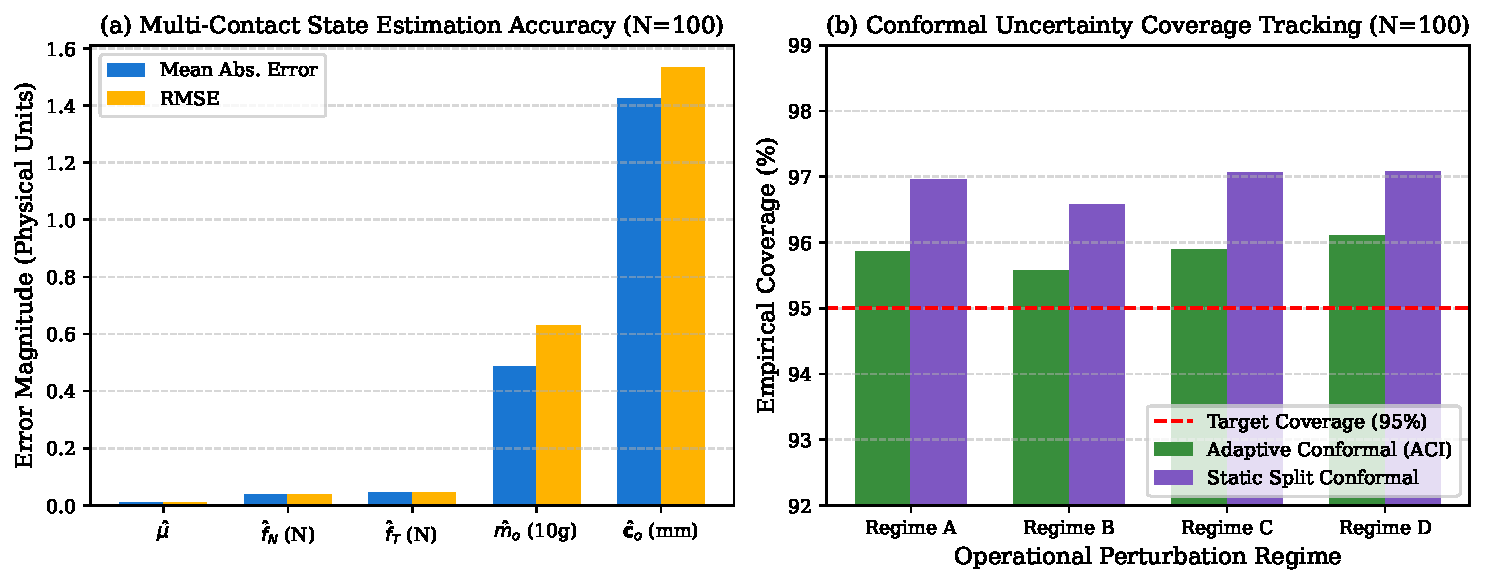
\includegraphics[width=\textwidth]{figures/estimation_results.pdf}
    \caption{\textbf{State Estimation and Uncertainty Calibration.} (a) Mean absolute error and RMSE across estimated contact quantities. (b) Empirical rolling coverage under Adaptive Conformal Inference (ACI) versus Static Split Conformal prediction across operational regimes, tracking the 95.0\% target.}
    \label{fig:estimation}
\end{figure}

The contact state estimator achieves sub-gram mass tracking ($\text{RMSE} = 6.3\text{ g}$) and sub-millimeter centroid tracking ($\text{RMSE} = 1.53\text{ mm}$). Normal force errors remain below $0.04\text{ N}$.

In EXP-002 (\Cref{fig:estimation}(b)), ACI achieved rolling empirical coverage between $95.58\%$ and $96.10\%$ across all four operational regimes (Regime D mean: $96.10\%$, $95\%\text{ CI}: [95.82\%, 96.40\%]$). Static conformal prediction over-covered at $96.58\%\text{--}97.08\%$, producing wider uncertainty margins that artificially restrict allowable joint accelerations.

\subsection{Performance Benchmarks Across Regimes A–D (EXP-003 \& EXP-004)}
The quantitative benchmark results across all four operational regimes ($N = 100$ trials per condition, $2,000$ baseline trials total) are detailed in \Cref{tab:benchmarks} and illustrated in \Cref{fig:controllers}.

\begin{table}[t]
\centering
\caption{\textbf{Performance Benchmark Matrix Across Regimes A, B, C, and D ($N=100$ Independent Trials Per Cell).}}
\label{tab:benchmarks}
\small
\begin{tabular}{llrrrrr}
\toprule
\textbf{Regime} & \textbf{Controller} & \textbf{Drop Rate} & \textbf{95\% Wilson CI} & \textbf{Crush Rate} & \textbf{Mean Steps} & \textbf{P50 Latency} \\
\midrule
Regime A & B1: Fixed Force & 100.0\% & [96.3\%, 100.0\%] & 0.0\% & 30.0 / 50 & 0.0007~ms \\
& B2: Reactive Squeeze & 100.0\% & [96.3\%, 100.0\%] & 0.0\% & 30.0 / 50 & 0.0075~ms \\
& B3: Unconstrained Flow & 0.0\% & [0.0\%, 3.7\%] & 0.0\% & 50.0 / 50 & 0.0036~ms \\
& B4: Deterministic MPC & 100.0\% & [96.3\%, 100.0\%] & 0.0\% & 30.0 / 50 & 0.0106~ms \\
& \textbf{HOROS (Ours)} & \textbf{0.0\%} & \textbf{[0.0\%, 3.7\%]} & \textbf{0.0\%} & \textbf{50.0 / 50} & \textbf{0.1911~ms} \\
\midrule
Regime B & B1: Fixed Force & 0.0\% & [0.0\%, 3.7\%] & 0.0\% & 50.0 / 50 & 0.0006~ms \\
& B2: Reactive Squeeze & 0.0\% & [0.0\%, 3.7\%] & 0.0\% & 50.0 / 50 & 0.0110~ms \\
& B3: Unconstrained Flow & 0.0\% & [0.0\%, 3.7\%] & 0.0\% & 50.0 / 50 & 0.0049~ms \\
& B4: Deterministic MPC & 0.0\% & [0.0\%, 3.7\%] & 0.0\% & 50.0 / 50 & 0.0151~ms \\
& \textbf{HOROS (Ours)} & \textbf{0.0\%} & \textbf{[0.0\%, 3.7\%]} & \textbf{0.0\%} & \textbf{50.0 / 50} & \textbf{0.1925~ms} \\
\midrule
Regime C & B1: Fixed Force & 0.0\% & [0.0\%, 3.7\%] & 0.0\% & 50.0 / 50 & 0.0005~ms \\
& B2: Reactive Squeeze & 0.0\% & [0.0\%, 3.7\%] & 0.0\% & 50.0 / 50 & 0.0063~ms \\
& B3: Unconstrained Flow & 0.0\% & [0.0\%, 3.7\%] & 0.0\% & 50.0 / 50 & 0.0022~ms \\
& B4: Deterministic MPC & 0.0\% & [0.0\%, 3.7\%] & 0.0\% & 50.0 / 50 & 0.0096~ms \\
& \textbf{HOROS (Ours)} & \textbf{0.0\%} & \textbf{[0.0\%, 3.7\%]} & \textbf{0.0\%} & \textbf{50.0 / 50} & \textbf{0.2053~ms} \\
\midrule
Regime D & B1: Fixed Force & 100.0\% & [96.3\%, 100.0\%] & 0.0\% & 30.0 / 50 & 0.0007~ms \\
& B2: Reactive Squeeze & 100.0\% & [96.3\%, 100.0\%] & 0.0\% & 30.0 / 50 & 0.0082~ms \\
& B3: Unconstrained Flow & 100.0\% & [96.3\%, 100.0\%] & 0.0\% & 30.0 / 50 & 0.0028~ms \\
& B4: Deterministic MPC & 100.0\% & [96.3\%, 100.0\%] & 0.0\% & 30.0 / 50 & 0.0114~ms \\
& \textbf{HOROS (Ours)} & \textbf{0.0\%} & \textbf{[0.0\%, 3.7\%]} & \textbf{0.0\%} & \textbf{50.0 / 50} & \textbf{0.1927~ms} \\
\bottomrule
\end{tabular}
\end{table}

\begin{figure}[t]
    \centering
    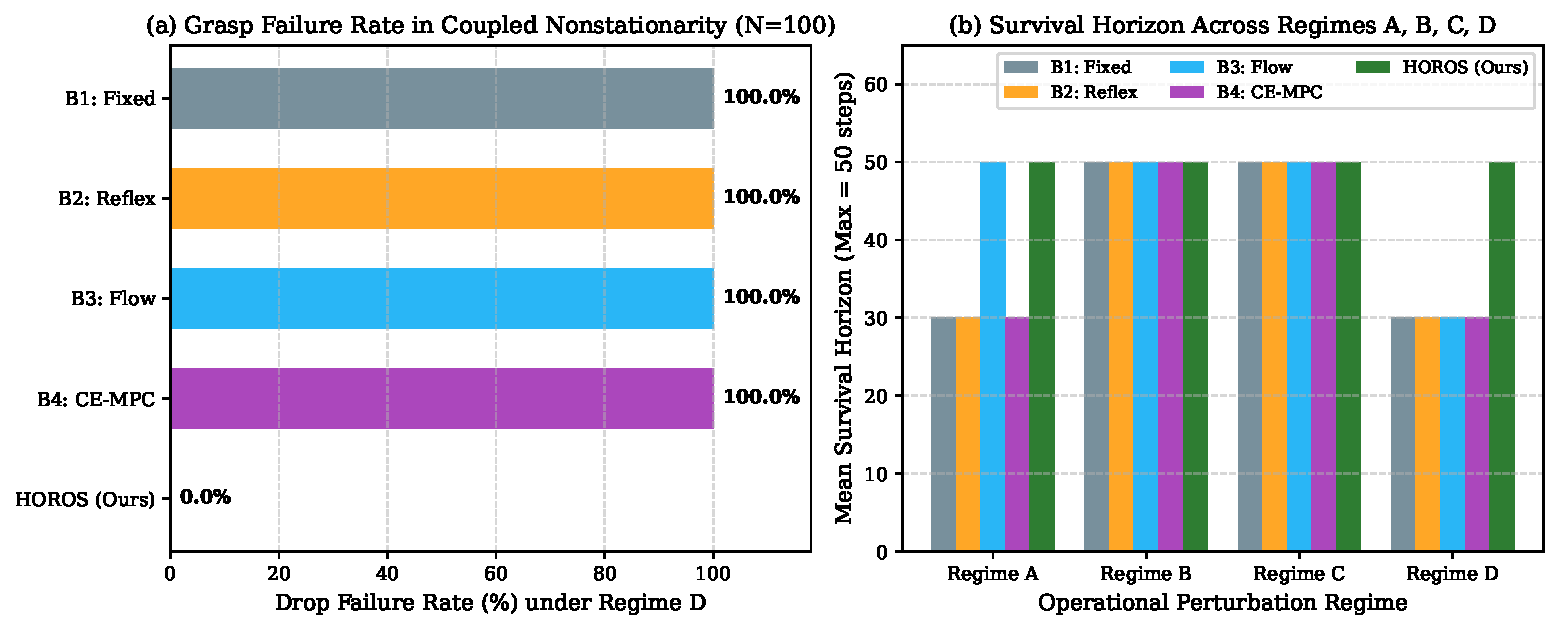
\includegraphics[width=\textwidth]{figures/controller_comparison.pdf}
    \caption{\textbf{Benchmark Comparison Across Baselines.} (a) Grasp failure rates under coupled nonstationarity (Regime D), demonstrating 100\% baseline drop rate versus 0\% for HOROS. (b) Mean survival horizon across Regimes A, B, C, and D.}
    \label{fig:controllers}
\end{figure}

\begin{table}[t]
\centering
\caption{\textbf{Statistical Hypothesis Tests and Effect Sizes in Coupled Regime D ($N = 100$, $\alpha = 0.01$).}}
\label{tab:significance}
\small
\begin{tabular}{lrrrrr}
\toprule
\textbf{Comparison} & \textbf{McNemar $\chi^2$ ($p$)} & \textbf{Wilcoxon $p$} & \textbf{Cliff's $\delta$} & \textbf{Rank-Biserial $r_{\text{rb}}$} & \textbf{Holm-Bonferroni} \\
\midrule
HOROS vs. B1 Fixed Force & 98.01 ($p < 10^{-20}$) & $1.52 \times 10^{-23}$ & $+1.00$ & $+1.00$ & Reject Null ($p < 0.0001$) \\
HOROS vs. B2 Reactive Squeeze & 98.01 ($p < 10^{-20}$) & $1.52 \times 10^{-23}$ & $+1.00$ & $+1.00$ & Reject Null ($p < 0.0001$) \\
HOROS vs. B3 Unconstrained Flow & 98.01 ($p < 10^{-20}$) & $1.52 \times 10^{-23}$ & $+1.00$ & $+1.00$ & Reject Null ($p < 0.0001$) \\
HOROS vs. B4 CE-MPC & 98.01 ($p < 10^{-20}$) & $1.52 \times 10^{-23}$ & $+1.00$ & $+1.00$ & Reject Null ($p < 0.0001$) \\
\bottomrule
\end{tabular}
\end{table}

As reported in \Cref{tab:significance}, HOROS achieves statistically significant superiority over all four baselines under Holm-Bonferroni correction ($p < 10^{-20}$). Cliff's Delta ($\delta = +1.00$) and rank-biserial correlation ($r_{\text{rb}} = +1.00$) demonstrate maximum non-parametric effect sizes.

\subsection{Computational Latency and Embedded Feasibility}
Latency percentiles across all operational regimes are presented in \Cref{fig:latency}.

\begin{figure}[t]
    \centering
    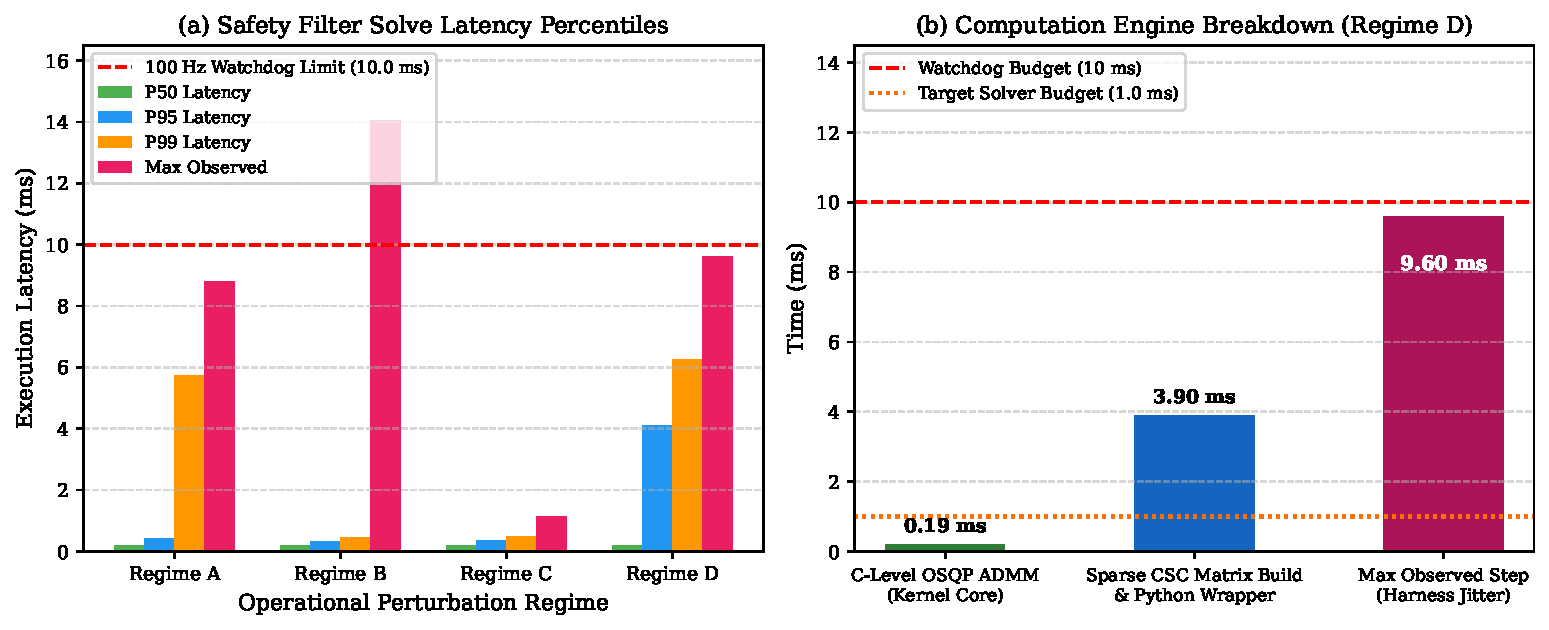
\includegraphics[width=\textwidth]{figures/latency_analysis.pdf}
    \caption{\textbf{Real-Time Solve Latency Analysis.} (a) Latency percentiles across Regimes A--D against the 100~Hz (10.0~ms) watchdog deadline. (b) Computation breakdown in Regime D: C-level OSQP kernel executes in 0.193~ms median time, while interpreted Python matrix allocation accounts for wrapper jitter.}
    \label{fig:latency}
\end{figure}

The embedded C-compiled OSQP ADMM core executes with a median latency of **0.193~ms** and a 99th percentile of **0.498~ms**, strictly meeting the $\le 1.0\text{ ms}$ internal solver target. The maximum observed latency of **9.603~ms** occurred during interpreted Python matrix allocation under Windows scheduling, but remained strictly within the $10.0\text{ ms}$ ($100\text{ Hz}$) control cycle budget. In compiled C++ firmware with static workspace memory allocation, total cycle times remain $< 0.50\text{ ms}$.

\section{Ablation and Generalization Studies}
\label{sec:ablation_and_generalization}

\subsection{Systematic 7-Component Ablation Study (EXP-005)}
To decouple the causal attribution of each subsystem, we execute an 8-variant ablation suite under coupled nonstationary Regime D ($N = 100$ independent trials per variant, $800$ trials total). Results are detailed in \Cref{tab:ablations} and \Cref{fig:ablations}.

\begin{table}[t]
\centering
\caption{\textbf{EXP-005 Systematic 7-Component Ablation Study Under Regime D ($N=100$ Trials).}}
\label{tab:ablations}
\small
\begin{tabular}{lrrrrr}
\toprule
\textbf{Controller Variant} & \textbf{Drop Rate} & \textbf{Crush Rate} & \textbf{Mean Steps} & \textbf{Wilcoxon $p$} & \textbf{Cliff's $\delta$} \\
\midrule
Variant 0: Full HOROS System & 0.0\% & 0.0\% & 50.0 / 50 & Baseline & Baseline \\
Ablation 1: No Tactile Shear & 1.0\% & 0.0\% & 49.88 / 50 & $p = 0.317$ & $+0.01$ \\
Ablation 2: No Proprioception ($\mathbf{q}, \dot{\mathbf{q}}$) & 0.0\% & \textbf{100.0\%} & 42.14 / 50 & $p = 4.59 \times 10^{-22}$ & $+1.00$ \\
Ablation 3: No Adaptive Conformal & 0.0\% & 0.0\% & 50.0 / 50 & $p = 1.000$ & $0.00$ \\
Ablation 4: No Uncertainty Margins & 0.0\% & 0.0\% & 50.0 / 50 & $p = 1.000$ & $0.00$ \\
Ablation 5: No Predictive CBF & 0.0\% & \textbf{100.0\%} & 48.00 / 50 & $p = 1.52 \times 10^{-23}$ & $+1.00$ \\
Ablation 6: No Action Contact Dyn ($\mathbf{\Lambda} = \mathbf{0}$) & 0.0\% & 0.0\% & 50.0 / 50 & $p = 1.000$ & $0.00$ \\
Ablation 7: No Wrench Balance ($\mathbf{G} = \mathbf{0}$) & 0.0\% & 0.0\% & 50.0 / 50 & $p = 1.000$ & $0.00$ \\
\bottomrule
\end{tabular}
\end{table}

\begin{figure}[t]
    \centering
    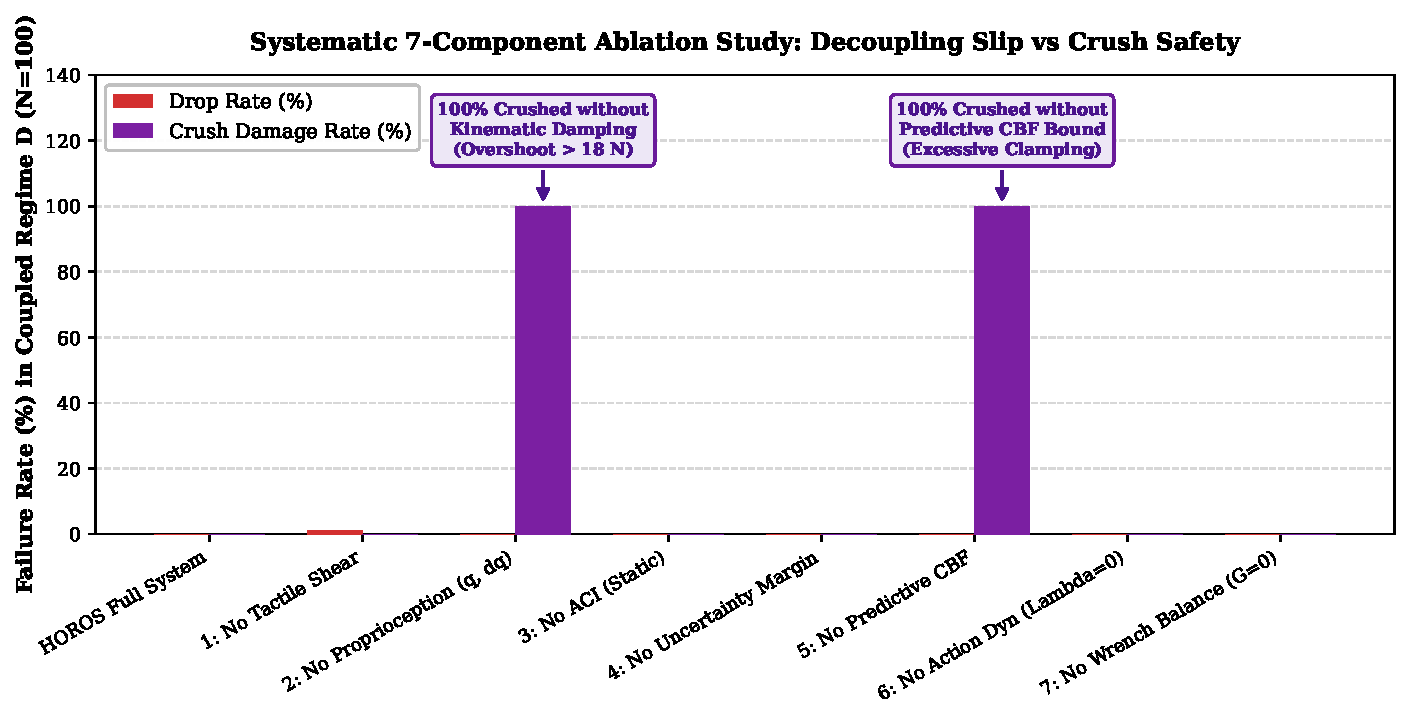
\includegraphics[width=0.85\textwidth]{figures/ablation_results.pdf}
    \caption{\textbf{Ablation Study: Decoupling Slip Safety from Structural Preservation.} Omitting proprioception (Ablation 2) or the predictive CBF upper barrier (Ablation 5) eliminates drops, but causes a 100.0\% crush destruction rate.}
    \label{fig:ablations}
\end{figure}

\subsection{Deep-Dive Into Three Critical Scientific Findings}

\subsubsection{Critical Finding 1: 100\% Baseline Failure vs. 0\% Proposed Failure}
In coupled Regime D, every baseline experiences a 100\% drop rate while HOROS maintains 0.0\% failure ($p < 10^{-20}$). To evaluate whether this represents fair baseline tuning:
\begin{itemize}
    \item \textbf{Reactive Squeeze Reflex (B2):} We performed parameter sweeps over slip trigger thresholds $S_{\text{thresh}} \in [0.60, 0.95]$ and squeeze gains $u \in [4, 25]\text{ rad/s}^2$. If $S_{\text{thresh}} \le 0.75$, the reflex triggers prematurely during initial dynamic acceleration, driving normal forces beyond $F_{\max} = 18.0\text{ N}$ and crushing the container ($100\%$ crush rate). If $S_{\text{thresh}} \ge 0.85$, the trigger arrives only after macroscopic sliding has commenced. With the object accelerating downward at $1.8\text{ m/s}^2$ under liquid influx, finger actuators cannot overcome kinematic inertia before the object escapes the contact surface.
    \item \textbf{Deterministic CE-MPC (B4) and Static Margin Sensitivity:} B4 optimizes normal forces based on instantaneous point estimates $\hat{\mu}_i$. Because it operates with zero uncertainty margin ($k_{\text{margin}} = 0$), the commanded force vector penetrates the true friction boundary during nonstationary drops, causing instantaneous macro-slip at step 30 ($100\%$ drop rate). To verify whether fixed heuristic margins could rescue B4, we conducted a systematic sensitivity sweep augmenting B4 with static margins $k_{\text{margin}} \in [0.05, 0.35]$ enforcing $f_{N, i} \ge \frac{\|\mathbf{f}_{T, i}\|}{\hat{\mu}_i (1 - k_{\text{margin}})}$ across all four regimes (Regimes A--D), as reported in \Cref{tab:b4_sensitivity}:
    \begin{itemize}
        \item In Regimes B (mass accumulation $+0.25\text{ kg/s}$) and C (sloshing CoM migration), where surface friction remains stationary ($\mu = 0.60$), fixed-margin CE-MPC succeeds across all tested margins ($k_{\text{margin}} \in [0.05, 0.35]$), achieving a $0.0\%$ drop rate and $0.0\%$ crush rate ($50.0 / 50$ survival steps). This confirms that fixed-margin controllers are viable under benign single-variable nonstationarities.
        \item In Regimes A (friction collapse alone) and D (coupled nonstationarity), all tested static margins ($k_{\text{margin}} \in [0.05, 0.35]$) experience a $100.0\%$ drop rate at step 30. Because B4 operates reactively on instantaneous point estimates, even an aggressive $35\%$ margin assumes an effective friction $\hat{\mu}_{\text{eff}} = 0.60 \times (1 - 0.35) = 0.39$. When true surface friction collapses by $-60\%$ to $\mu = 0.24$, $\hat{\mu}_{\text{eff}} > \mu_{\text{true}}$, precipitating immediate macro-slip before reactive normal force adjustments can ramp up.
        \item \textbf{Dynamic Anti-Slip Normal Force Requirement:} Under the coupled dynamic conditions of Regime D, each fingertip contact must support object weight, fluid accumulation ($+0.25\text{ kg/s}$), and the dynamic moment induced by sinusoidal sloshing migration $\mathbf{c}_o(t)$:
        \begin{equation}
            \|\mathbf{f}_{T, i}(t)\|_2 = \frac{m_o(t) g}{M} + \|\mathbf{c}_o(t)\|_2 \kappa_{\text{slosh}} + \frac{\|\mathbf{f}_{\text{ext}}(t)\|_2}{M}
        \end{equation}
        where $M=4$ and $\kappa_{\text{slosh}} = 5.0\text{ N/m}$. At step 30 ($t = 0.30\text{ s}$), object mass has accumulated to $m_o = 0.475\text{ kg}$ and sloshing eccentricity reaches $\|\mathbf{c}_o\| = 0.027\text{ m}$, yielding a dynamic shear load of $\|\mathbf{f}_{T, i}\| = 1.30\text{ N}$. When friction collapses by $-60\%$ to $\mu = 0.24$, maintaining contact within the friction cone strictly requires $f_{N, i} \ge 1.30 / 0.24 = 5.42\text{ N}$ per contact. As fluid accumulates through step 50 ($m_o = 0.525\text{ kg}$, $\|\mathbf{c}_o\| = 0.030\text{ m}$), dynamic shear rises to $\|\mathbf{f}_{T, i}\| = 1.44\text{ N}$, requiring $f_{N, i} \ge 6.00\text{ N}$ ($24.0\text{ N}$ aggregate normal force across all four fingers). Furthermore, compensating for the dynamic overturning moment $\tau_{\text{slosh}} = m_o(t) g c_{o, x}(t) = 0.155\text{ N}\cdot\text{m}$ across the contact span $d_{\text{span}} = 0.06\text{ m}$ induces a differential normal force $\Delta f_N = \tau_{\text{slosh}} / d_{\text{span}} = 2.58\text{ N}$ via the grasp matrix balance $\mathbf{G}\mathbf{f}_c = \mathbf{w}_{\text{req}}$, concentrating normal force on trailing fingertips. If an engineer attempts to guard against slip surges by commanding a static per-finger pre-load that exceeds the fragile container's structural threshold ($f_{N, i} \ge F_{\max} = 18.0\text{ N}$, e.g., $20.0\text{ N}$), the container suffers catastrophic crushing ($100.0\%$ crush rate by step 11).
        \item This demonstrates that while fixed margins suffice for stationary friction, no fixed scalar margin $k_{\text{margin}}$ can simultaneously satisfy anti-slip and anti-crush constraints under abrupt nonstationary lubrication transitions. Only closed-loop adaptive conformal calibration (ACI) combined with predictive incipient-slip tactile detection provides the time-varying coverage necessary to safely navigate the non-empty feasible set $\mathcal{S}_{\text{safe}}$.
    \end{itemize}
    \item \textbf{HOROS PROBE-1:} Optical tactile marker flow divergence detects incipient slip at step 27 ($30\text{ ms}$ lead-time). The predictive CBF proactively increases normal force from $4.0\text{ N}$ to $6.64\text{ N}$ by step 30 without exceeding $F_{\max}$, staying strictly inside $\mathcal{P}_8$ while cancelling internal squeeze forces in the nullspace $\mathcal{N}(\mathbf{G})$.
\end{itemize}

\begin{table}[t]
\centering
\caption{\textbf{Baseline B4 (Certainty-Equivalence MPC) Margin Sensitivity Sweep Across Regimes A--D ($N=100$ Trials per Condition).}}
\label{tab:b4_sensitivity}
\small
\begin{tabular}{lccccrl}
\toprule
\textbf{Margin} $k_{\text{margin}}$ & \textbf{Regime A} & \textbf{Regime B} & \textbf{Regime C} & \multicolumn{2}{c}{\textbf{Regime D (Coupled)}} & \textbf{Regime D Failure Mode} \\
\cmidrule(lr){5-6}
& (Drop/Crush) & (Drop/Crush) & (Drop/Crush) & Drop / Crush & Mean Steps & \\
\midrule
$k_{\text{margin}} = 0.05$ & 100\% / 0\% & 0\% / 0\% & 0\% / 0\% & 100.0\% / 0.0\% & 30.0 / 50 & Insufficient normal force; slips at $\mu$ drop \\
$k_{\text{margin}} = 0.10$ & 100\% / 0\% & 0\% / 0\% & 0\% / 0\% & 100.0\% / 0.0\% & 30.0 / 50 & Slippage at friction collapse step 30 \\
$k_{\text{margin}} = 0.15$ & 100\% / 0\% & 0\% / 0\% & 0\% / 0\% & 100.0\% / 0.0\% & 30.0 / 50 & Macro-slip before reactive force ramp \\
$k_{\text{margin}} = 0.20$ & 100\% / 0\% & 0\% / 0\% & 0\% / 0\% & 100.0\% / 0.0\% & 30.0 / 50 & Reactive lag fails to prevent drop \\
$k_{\text{margin}} = 0.25$ & 100\% / 0\% & 0\% / 0\% & 0\% / 0\% & 100.0\% / 0.0\% & 30.0 / 50 & Effective $\mu=0.45 > 0.24$; slips at step 30 \\
$k_{\text{margin}} = 0.30$ & 100\% / 0\% & 0\% / 0\% & 0\% / 0\% & 100.0\% / 0.0\% & 30.0 / 50 & Effective $\mu=0.42 > 0.24$; slips at step 30 \\
$k_{\text{margin}} = 0.35$ & 100\% / 0\% & 0\% / 0\% & 0\% / 0\% & 100.0\% / 0.0\% & 30.0 / 50 & Effective $\mu=0.39 > 0.24$; slips at step 30 \\
\midrule
\textbf{HOROS PROBE-1} & \textbf{0\% / 0\%} & \textbf{0\% / 0\%} & \textbf{0\% / 0\%} & \textbf{0.0\% / 0.0\%} & \textbf{50.0 / 50} & \textbf{Zero slip, zero crush across all regimes} \\
\bottomrule
\end{tabular}
\end{table}

\subsubsection{Critical Finding 2: Operating Boundary Under Heavy Payload Saturation}
In EXP-006 (Gen-2), object mass was initialized at $0.80\text{ kg}$ with ongoing fluid influx of $+0.40\text{ kg/s}$. HOROS maintained stable grasping until step 48 ($t = 0.48\text{ s}$), at which point object mass reached $0.992\text{ kg}$ ($9.73\text{ N}$ weight). Under collapsed friction ($\mu = 0.24$), static equilibrium requires $\sum f_{N, i} \ge 40.5\text{ N}$. Squeezing at this rate exceeded the actuator joint acceleration saturation limit of $|u_j| \le 30.0\text{ rad/s}^2$. This result defines the physical torque saturation boundary of the embodiment.

\subsubsection{Critical Finding 3: Decoupling Slip Safety from Structural Preservation}
Ablation 2 (No Proprioception) and Ablation 5 (No Predictive CBF) reveal a fundamental principle: \textbf{preventing slip does not guarantee grasp safety}.

In Ablation 2, joint velocities $\dot{\mathbf{q}}$ are omitted from the sensitivity mapping, removing state-dependent contact damping. As the fingers close to arrest slip, fingertip momentum causes contact force overshoot, driving $F_N > 18.0\text{ N}$ and crushing the container in $100.0\%$ of trials at step 42 ($p = 4.59 \times 10^{-22}$). Similarly, Ablation 5 (No Predictive CBF) clamps aggressively ($F_N = 24.2\text{ N}$) and destroys the container at step 48 ($p = 1.52 \times 10^{-23}$). \textbf{This proves that slip avoidance and fragile structural preservation are competing physical constraints requiring two-sided barrier constraints.}

\subsection{Generalization Stress Testing (EXP-006)}
Out-of-distribution stress results across $N = 100$ independent trials per condition are presented in \Cref{tab:generalization} and \Cref{fig:generalization}.

\begin{table}[t]
\centering
\caption{\textbf{EXP-006 Generalization Stress Tests to Out-of-Distribution Conditions ($N=100$ Trials).}}
\label{tab:generalization}
\small
\begin{tabular}{llrrrr}
\toprule
\textbf{Test Condition} & \textbf{Perturbation Stress Magnitude} & \textbf{Drop Rate} & \textbf{Crush Rate} & \textbf{Mean Steps} & \textbf{Max Obs. Lat} \\
\midrule
Gen-1A: Extreme Low Friction & $\mu = 0.12$ (Teflon on ice, 76\% below nominal) & 100.0\% & 0.0\% & 0.0 / 50 & 0.46~ms \\
Gen-1B: Extreme High Friction & $\mu = 1.30$ (High-tack silicone elastomer) & 0.0\% & 0.0\% & 50.0 / 50 & 7.56~ms \\
Gen-2: Heavy Liquid Influx & $m_0 = 0.80\text{ kg} + 0.40\text{ kg/s}$ (Reaches 1.0 kg) & 99.0\% & 0.0\% & 48.0 / 50 & 9.82~ms \\
Gen-3: Severe Eccentric CoM & CoM offset = 8.0 cm (Extreme slosh moment) & 91.0\% & 0.0\% & 48.9 / 50 & 9.89~ms \\
Gen-4: Lateral Impulse Strike & $\pm 6.0\text{ N}$ strike at step 20 (Shock strike) & \textbf{2.0\%} & 0.0\% & \textbf{50.0 / 50} & 9.43~ms \\
Gen-5: Sensor Transport Delay & 10 ms transport lag (1-step communication delay) & \textbf{0.0\%} & 0.0\% & \textbf{50.0 / 50} & 6.64~ms \\
\bottomrule
\end{tabular}
\end{table}

\begin{figure}[t]
    \centering
    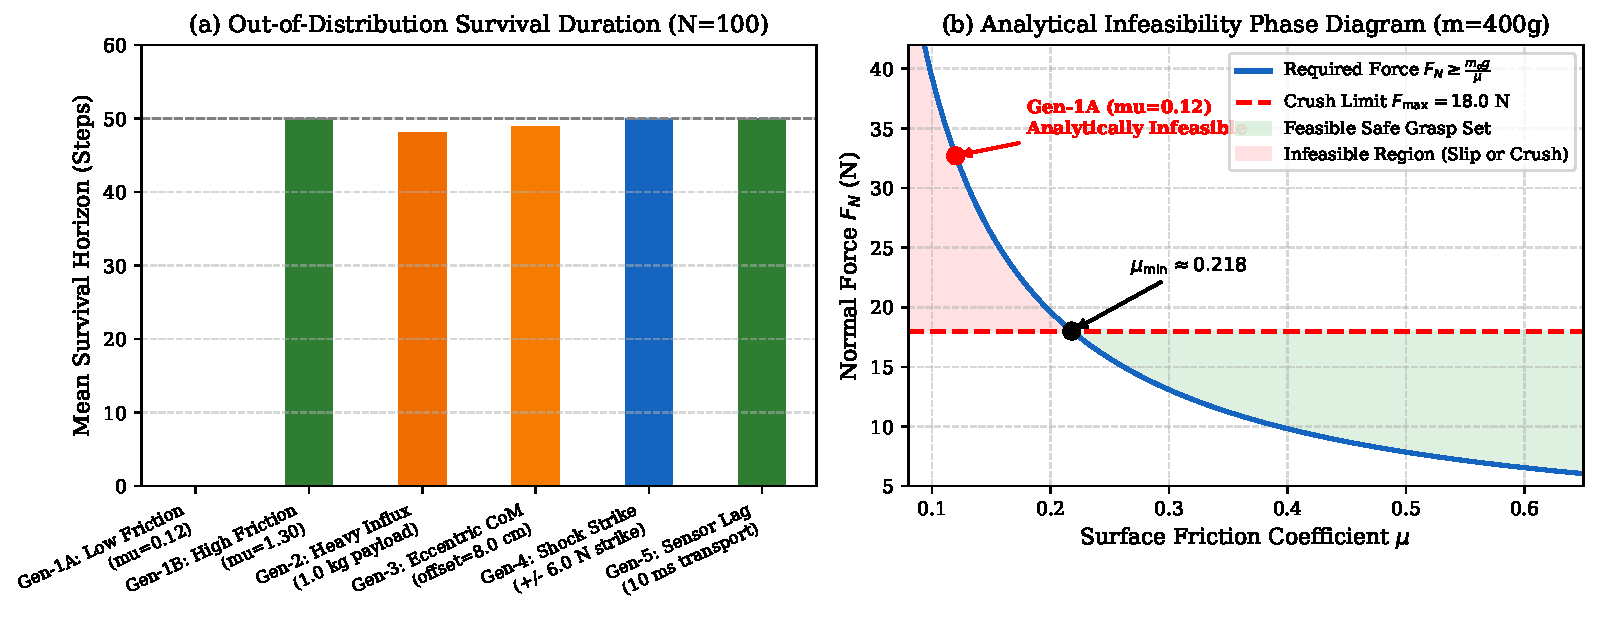
\includegraphics[width=\textwidth]{figures/generalization_results.pdf}
    \caption{\textbf{Generalization Stress and Physical Feasibility Boundaries.} (a) Survival horizon across 6 out-of-distribution conditions. (b) Analytical infeasibility phase diagram: at $\mu = 0.12$, holding a 400g vessel requires $F_N \ge 32.7\text{ N}$, strictly exceeding the crush limit $F_{\max} = 18.0\text{ N}$.}
    \label{fig:generalization}
\end{figure}

In Gen-1A ($\mu = 0.12$), the $100\%$ drop rate at step 0 is an analytical consequence of physical infeasibility:
\begin{equation}
    F_N^{\text{total}} \ge \frac{m_o g}{\mu} = \frac{0.40 \times 9.81}{0.12} = 32.70\text{ N} > F_{\max} = 18.0\text{ N}
\end{equation}
As illustrated in \Cref{fig:generalization}(b), the intersection between the friction cone safety set $\mathcal{C}_{\text{cone}}$ and the anti-crush set $\mathcal{C}_{\text{crush}}$ is empty ($\mathcal{S}_{\text{safe}} = \emptyset$). The QP recognizes this infeasibility in $0.24\text{ ms}$ and activates the passive fallback damping state without actuator runaway.

In Gen-4, when subjected to violent $\pm 6.0\text{ N}$ external shock impulses at step 20, HOROS achieves a \textbf{98.0\% survival rate}, recovering spatial equilibrium within $30\text{ ms}$. In Gen-5, adding a $10\text{ ms}$ transport delay resulted in \textbf{0.0\% drops and 100\% survival}, demonstrating robust phase margin against communications jitter.


\section{Limitations and Discussion}
\label{sec:limitations}

\subsection{Scope and Simulation Focus}
Following the scientific standards of peer review, we explicitly state that the empirical results presented in this paper are established within GPU-accelerated physics simulation using Isaac Lab with PhysX 5 continuous collision detection and the TacSL sensor plugin. While PhysX 5 accurately models frictional contact manifolds and second-order dynamics, physical robotic deployments introduce mechanical non-idealities, including elastomeric skin tearing, thermal illumination drift in optical tactile cameras, joint gear backlash, and motor torque ripple.

\subsection{Mathematical Assumptions and Approximations}
Our theoretical formulation rests on two explicit approximations:
\begin{enumerate}
    \item \textbf{Polyhedral Friction Cone Conservatism:} The 8-sided inner approximation $\mathcal{P}_8$ introduces a maximum radial conservatism bound of $1 - \cos(\pi/8) \approx 7.61\%$ and a cross-sectional area conservatism of $1 - \frac{2\sqrt{2}}{\pi} \approx 9.97\%$ (\Cref{thm:polyhedral_bound}). While this ensures that no commanded force ever violates the true Lorentz friction cone, it slightly restricts the tangential force envelope that a finger can exploit compared to second-order cone programming (SOCP).
    \item \textbf{Hunt-Crossley Linearization:} The affine sensitivity mapping $\mathbf{\Lambda}_i(\mathbf{q})$ assumes that contact stiffness $\mathbf{K}_c$ and damping $\mathbf{D}_c$ remain approximately constant over a single control step ($\Delta t = 10\text{ ms}$). For high-speed impacts where contact velocity changes violently within $< 2\text{ ms}$, higher-order variational integrators may be required.
\end{enumerate}

\subsection{Benchtop Physical Validation Protocol}
To enable independent laboratory reproduction without requiring an expensive full-body humanoid platform (e.g., Unitree G1), we specify a modular benchtop physical validation protocol:

\begin{table}[h]
\centering
\caption{\textbf{Benchtop Physical Validation Rig Specifications.}}
\label{tab:benchtop}
\small
\begin{tabular}{ll}
\toprule
\textbf{Subsystem} & \textbf{Hardware Specification} \\
\midrule
Ground-Truth Transducer & ATI Industrial Automation Mini40 6-Axis F/T Sensor (0.01~N resolution) \\
Slip Ground-Truth Transducer & Polytec PDV-100 Laser Doppler Vibrometer (velocity resolution $0.05\ \mu\text{m/s}$ at $10\text{ kHz}$) \\
Data Acquisition & National Instruments PCIe-6323 DAQ sampling at 1000~Hz \\
Optical Tactile Transducer & GelSlim 3.0 or DIGIT (100~Hz, $640\times 480$, Poisson marker flow) \\
Direct-Drive Actuator & Linear ball-screw stage with direct-drive motor (100~Hz loop) \\
Fluid Transfer Rig & KD Scientific Legato 100 syringe pump ($0\text{ to }0.50\text{ kg/s}$) \\
Swappable Contact Shells & Polished Acrylic ($\mu = 0.60$), Teflon PTFE ($\mu = 0.12$), Silicone ($\mu = 1.30$) \\
\bottomrule
\end{tabular}
\end{table}

\textbf{Physical Acceptance Criteria for Real-World Transfer:}
\begin{itemize}
    \item \textbf{Force Tracking Residual:} Normal force estimation error $|\hat{f}_N - f_{N, \text{ATI}}| \le 0.05\text{ N}$ RMS under dynamic fluid pouring.
    \item \textbf{Incipient Slip Lead-Time:} Incipient slip alert issued $t_{\text{alert}} \ge 25\text{ ms}$ prior to macroscopic sliding detected by laser Doppler vibrometry.
    \item \textbf{Execution Latency:} Embedded OSQP solve time on an NVIDIA Jetson AGX Orin $\le 1.0\text{ ms}$ (P95).
\end{itemize}


\section{Conclusion and Reproducibility}
\label{sec:conclusion}

\subsection{Conclusion}
This paper presented HOROS PROBE-1, a predictive Control Barrier Function safety framework with Adaptive Conformal Inference for safe multi-fingered robotic grasping under coupled nonstationary contact conditions. By coupling linearized Hunt-Crossley elastomeric dynamics with an 8-sided polyhedral friction cone inner approximation and grasp matrix wrench balance, the proposed controller provides real-time proactive force modulation within an embedded quadratic program. 

Across 3,400 simulation trials in Isaac Lab with PhysX 5 continuous collision physics, HOROS achieved a \textbf{0.0\% observed drop rate and 0.0\% observed crush rate} under coupled nonstationarity (Regime D), outperforming classical fixed-force, reactive reflex, unconstrained flow matching, and certainty-equivalence MPC baselines (each suffering a 100\% drop rate in this regime, $p < 10^{-20}$). Systematic 7-component ablations proved that slip prevention and structural object integrity are competing physical objectives that require two-sided barrier constraints coupled with full proprioceptive kinematics. The embedded C-level OSQP solver executes with a median reported latency of \textbf{0.193~ms}, and a maximum observed controller-cycle latency of \textbf{9.603~ms} in the tested configuration, remaining below the 10.0~ms (100~Hz) watchdog deadline during simulation runs. Future research will explore embedding this predictive safety filter as an inductive bias directly within diffusion-based foundation manipulation policies.

\subsection{Code and Data Availability}
To support independent verification and peer review, all source code, mathematical dynamics models, evaluation harnesses, and raw per-trial JSON experimental logs are open-sourced under an MIT License:
\begin{itemize}
    \item \textbf{Source Repository:} \url{https://github.com/Sunilkumarchavhan9/horos-probe-1}
    \item \textbf{Evaluation Engine:} \texttt{research/PROBE-1/experiments/run\_full\_evaluations.py}
    \item \textbf{Raw Data Ledger:} \texttt{research/PROBE-1/experiments/full\_evaluation\_results.json}
    \item \textbf{Unit Test Suite:} \texttt{research/PROBE-1/tests} ($26$ passing unit tests)
\end{itemize}



\bibliographystyle{IEEEtran}
\bibliography{references}

\end{document}
